\chapter{Memory Analysis}
To get a better insight on how Hive uses memory, I needed to build a basic model when and why Hive's reserved memory grows. During my work, I mainly focused on HiveServer2. The first step toward the model building was to get basic knowledge about Hive's code base and the query compilation process. The query life cycle mentioned in the previous chapter helped, but I had to find those steps in the code. If I have these points I am able to start measuring and maybe find some memory wastes.

\section{Finding the measuring points}
Hive has around 2 million lines of code so locating the main steps of the query processing was challenging. 

As a starting point, the user enters a query in the client. At this point, I run Hive locally, so the simplest way for submitting queries against Hive was using Beeline command line client. HS2 gets the query through its Thrift interface. After this, the query goes to the \textit{Driver} class, which is the main class for executing queries.

The Driver has two methods that are important for me: run and runInternal. The run method gets called first, which basically just delegates to the runInternal method. These two functions return with a CommandProcessorResponse, once the compilation and execution are done. 

\noindent The runInternal does the two main steps:
\begin{itemize}
	\item Driver.compile: gets the command string and parses, analyses the query and generates the execution plan.
	\item Driver.execute: gets the execution plan and executes it on a specific engine (MapReduce, Spark or TEZ).
\end{itemize}

\subsection{Compile}
The first step of the compilation is the parsing. It takes a string and returns an Abstract Syntax Tree (AST or the Parse Tree).

\begin{lstlisting}
public int compile(String command, ...) {
...
	ASTNode tree;
	try {
		tree = ParseUtils.parse(command, ctx);
	} catch (ParseException e) {
...
}
\end{lstlisting}
\subsubsection{Semantic Analyzis}
After the AST is generated, the compile process will continue with the semantic analyzer. The type of the analyzer will depend on the query type we are running. For SELECT and INSERT the SemanticAnalyzer class is used. 

\begin{lstlisting}
public int compile(String command, ...) {
...
	BaseSemanticAnalyzer sem = SemanticAnalyzerFactory.get(queryState, tree);
...
	sem.analyze(tree, ctx);
...
}
\end{lstlisting}

The SemanticAnalyzer class is the main phase during compilation. It checks for semantic errors, fetches metadata from Metastore, generates and optimizes the query plan. The analyze method of the BaseSemanticAnalyzer is called from the Driver's compile method, and it delegates the call to the corresponding Analyzer. From now on, I will write about the SemanticAnalyzer class and its phases (which is executed for SELECTS and INSERTS.

\begin{lstlisting}
void analyzeInternal(ASTNode ast, PlannerContext plannerCtx) {
	//(1)
	if (!genResolvedParseTree(ast, plannerCtx)) {
		return;
	}
	//(2)
	Operator sinkOp = genOPTree(ast, plannerCtx);
	...
	//(3)
	...
	resultSchema = convertRowSchemaToViewSchema(...);
	...
	//(4)
	Optimizer optm = new Optimizer();
	... = optm.optimize();
	...
	//(5)
	TaskCompiler compiler = TaskCompilerFactory.getCompiler(conf, pCtx);
	compiler.compile(pCtx, rootTasks, inputs, outputs);
	...
}
\end{lstlisting}

\begin{enumerate}
	\item Fetches metadata and fill the Parse Tree with it so it becomes a Resolved Parse Tree.
	\item The Operation Tree gets created which will contain operators that process data read from the table. This tree is called by the Map and Reduce methods.
	\item The semantic analyzer will deduce the schema of the result set from the row schema
	\item A logical optimization is done on the Operator Tree. There are two types of optimization: one that transforms the Operator Tree (like removing unnecessary operations) and one that does not (predicate pushdown, vectorization \etc).
	\item Physical optimization and translation to the target execution engine take place. The output of this stage is the query plan. It can optimize the tree according to the engine used. For example in MR, common join can be translated to map-side join, if one of the tables is small enough to fit into the memory of the map nodes.
\end{enumerate}

\begin{lstlisting}
public int compile(String command, ...) {
	...
	sem.validate();
	...
}
\end{lstlisting}

After the semantic analysis is completed, the Driver will validate the plan. When it completes, the compilation ends and Hive will continue with the execution.

\clearpage
\section{Measure the memory of HiveServer2}
If I want to measure the memory usage of Hive, I need a something to create and analyze heap dumps and generate memory statistics. There are several tools to choose from. In this section, I will present the tools I considered and the method I used to get a better understanding of HS2 memory patterns.

\subsection{Tools for generating heap dumps and statistics}
For creating heap dumps and statistics of the memory, I decided to use a command line tool. In contrast of a UI tool, it has the benefits to generate heap dumps and statistics automatically. 

\subsubsection{jmap}
\textit{jmap} \cite{jmap} can be used to obtain heap dumps and histograms from a running java process.

To gather information about a running Java program we need its process ID (PID). Using this we can easily create the heap dump with the \textit{-dump} option. If we do not want to analyze large heap dumps, just to get the objects that reserve the most memory, we can use the \textit{-histo} option. It will print a histogram of the heap, containing each Java class, the number of objects and memory sizes per class.

\subsubsection{jcmd}
\textit{jmap} would have been a perfect choice for measuring memory. However, it is recommended to use the latest utility, which is called \textit{jcmd} \cite{jcmd}. It has enhanced diagnostics capability and its perfomance overhead is reduced. 

The usage of jcmd is similar to jmap. For creating heap dumps we can use \textit{jcmd <PID> GC.heap\_dump}. If we want to obtain class histogram we can do that with the \textit{jcmd <PID> GC.class\_histogram} command. With the \textit{jcmd <PID> GC.heap\_info} command we can gather basic information of the heap: \eg young and old memory of the process.

I decided to use jcmd in my future work to gather memory information automatically and generate heap dumps at the measuring points identified in the previous section.

\subsection{Tools for analysing heap dumps}
Creating heap dumps with a CLI tool is easier, however analysing those requires a tool with user interface. 

\subsubsection{YourKit}
\textit{YourKit} provides great analysing capabilities for heap dumps. We can use it for profiling local or remote Java applications. It has controllable overhead. Although, it is a great tool for profiling Java applications, it is a commercial software and only has 15 days of free licence.

\subsubsection{VisualVM}
\textit{VisualVM} provides a great visual interface for profiling Java applications and browsing heap dumps. It offers multiple views for analysing them. We can get the summary of the dump which contains the total bytes, classes and objects. 

With the "classes view" we can get information about the reserved memory and number of instances for each class. We can calculate the retained memory, which is the memory that would be freed if the objects would be garbage collected.

\subsubsection{JXRay}
JXRay \cite{jxray} is a memory analysis tool for Java applications. It creates a HTML report of a given heap dump. It can automatically detect common problems, like data duplication or non-optimal usse of data stuctures. 

JXRay can give us a compact report, even if the heap dump analyzed is 10's of GB. It can calculate how much memory taken by a collection internal representation and their workload, since JXRay knows about the internal representation of common java collections (HashMap, ArrayList \etc).

\begin{figure}[H]
	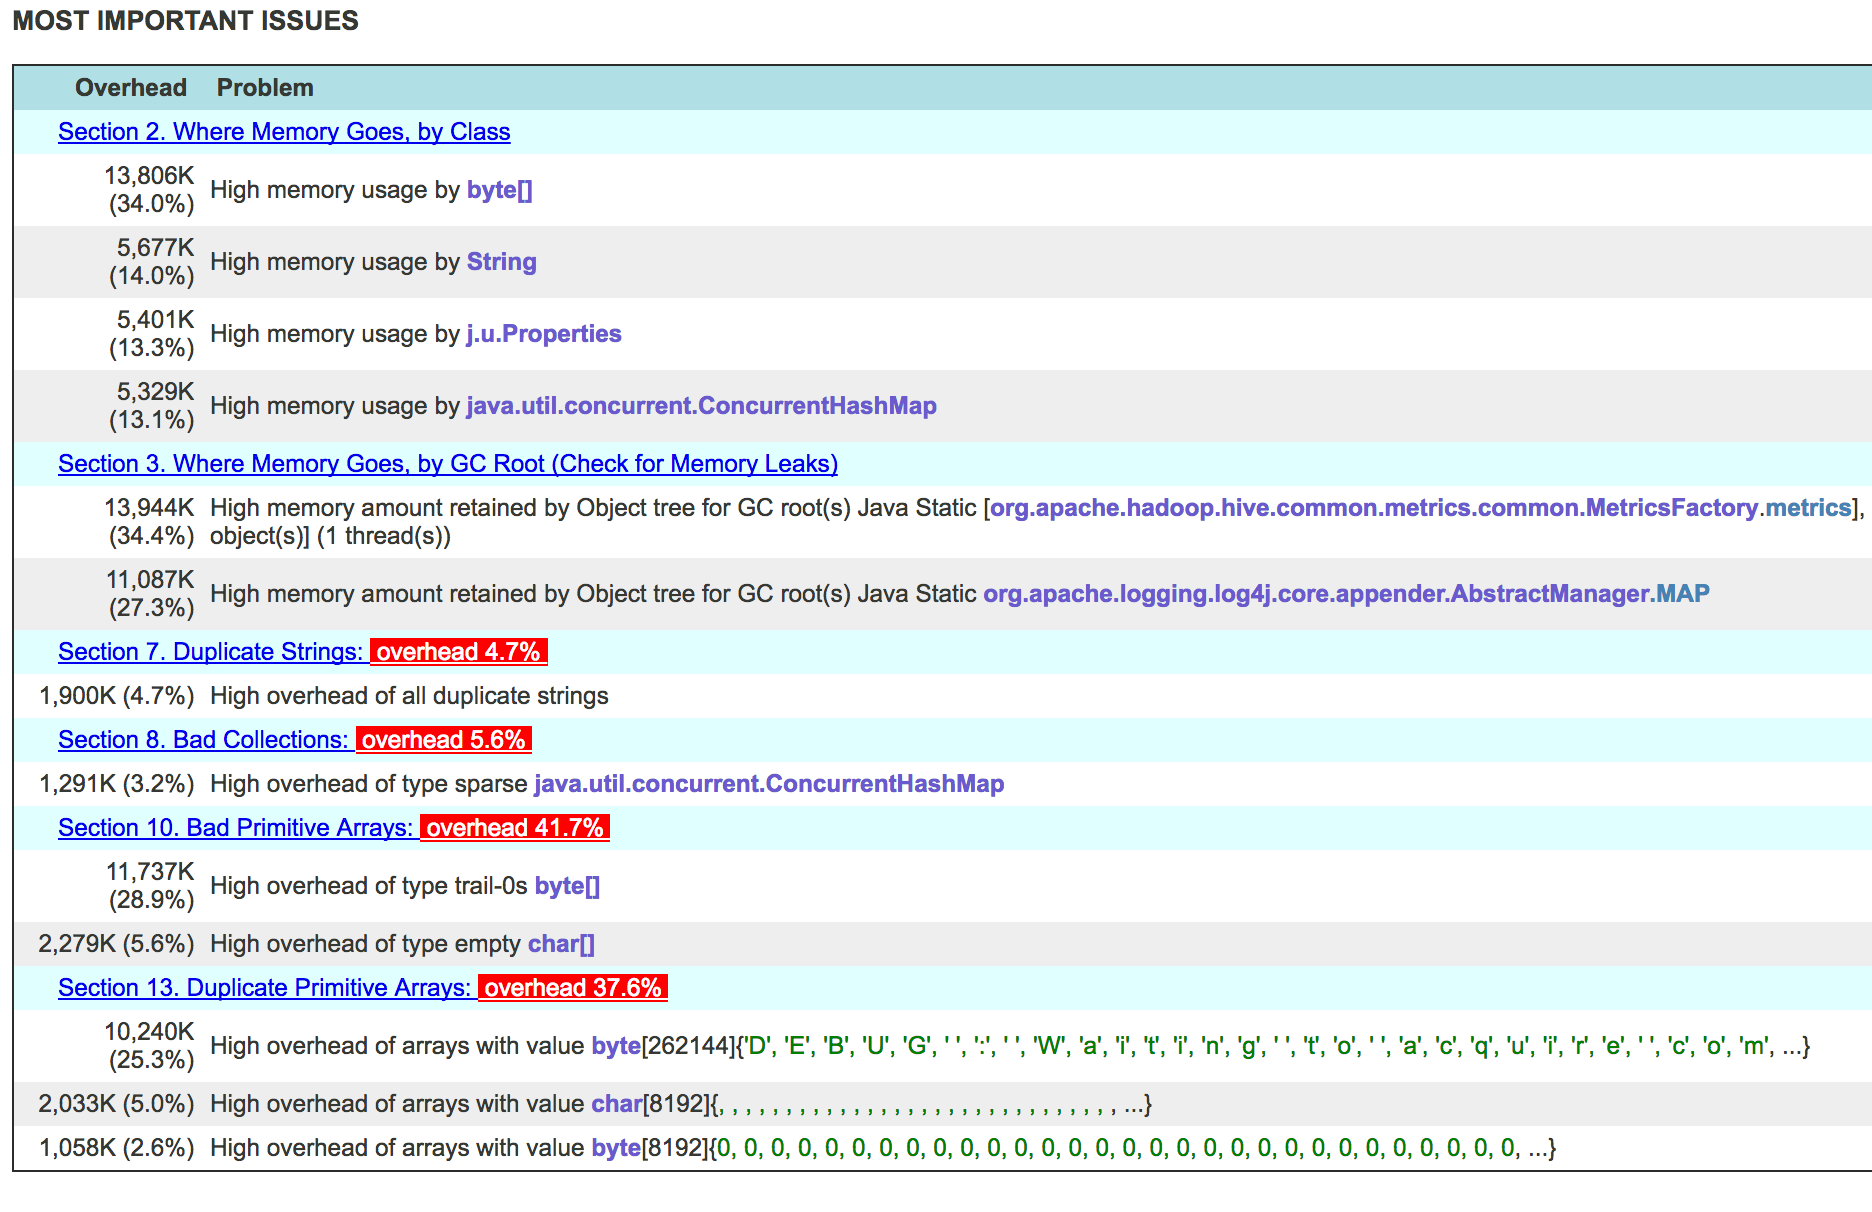
\includegraphics[width=150mm, keepaspectratio]{figures/jxray_sample.png}
	\centering
	\caption{Sample JXRay report summary}
\end{figure}

\subsubsection{The selected tool}
I decided to use VisualVM for visual memory analysis since it has great capabilities for summarizing the most important information about a heap dump and with its help, I am able to walk through the memory tree easily.

During my work, I also used JXRay, since it can automatically detect the most common memory problems and give me an overview of the possible issues a Java application has.

\clearpage
\subsection{Creating the code to measure memory}
With the available tools I am able to generate heap dumps really easily. However, to get a model how Hive uses the memory, I should gather statistics and heap dumps at certain points of the query execution. Clearly, it is not possible by hand. Thus, I needed to create a class in Hive's codebase and integrate the sampling in the identified points found in the previous section.

In order to use jcmd from Java, I needed a way to execute a terminal command from code. With the \textit{ProcessBuilder} java class I'm able to create operating system processes with the given attributes. The \textit{Runtime.exec()} method would do the same, but using this command is discouraged. 

Now that I can run a command line tool from Java, I will need the process ID of HiveServer2. Since Hive uses Java 8, I cannot use the new Process API that Java 9 provides. With the help of the \textit{ManagementFactory} class, we can get the managed bean of the runtime system of the JVM. It will return a class implementing the \textit{RuntimeMXBean} interface. The name of the running JVM contains the ID of the process. With the \textit{RuntimeMXBean.getName()} method, I was able to get the PID of HiveServer2. The method will return a string in a format of: \textit{pid@hostname}. Using the split method we can get our application's process ID.

To avoid code duplication I created a method for getting the ProcessBuilder which contains the given command and the PID for HiveServer2 is already set.

\begin{lstlisting}
private ProcessBuilder getProcessBuilder(String subCommand){
	ProcessBuilder builder = new ProcessBuilder();
	//Get own pid
	String pid = ManagementFactory.getRuntimeMXBean().getName().split("@")[0];
	builder.command("sh", "-c", String.format("jcmd %s %s", pid, subCommand));
	return builder;
}
\end{lstlisting}

Using the \textit{getProcessBuilder} function, it is really simple to run a terminal command. For example, getting information about the state of the heap or creating a heap dump will look like this:

\begin{lstlisting}
...
 process =  getProcessBuilder("GC.heap_info").start();
 ...
 getProcessBuilder("GC.heap_dump " + path).start();
\end{lstlisting}

\subsubsection{Parsing result}
I am able to create detailed statistics about the current memory state at certain phases of the query. As a first approach, I decided to just use \textit{GC.heap\_info} to see how memory usage looks like at different stages, not caring how much memory is reserved by each class. However, if we look at the result of the \textit{jcmd <PID> GC.heap\_info}, it will look quite messy, and hides the most important details, especially if we have 15 result for each query. An example how it looks:

\begin{lstlisting}
21566:
PSYoungGen total 1395200K, used 27419K [0x000000076ab00000, 0x00000007c0000000,
0x00000007c0000000)
eden space 1392640K, 1% used
[0x000000076ab00000,0x000000076c5c6c70,0x00000007bfb00000)
from space 2560K, 0% used [0x00000007bfd80000,0x00000007bfd80000,0x00000007c0000000)
to space 2560K, 0% used [0x00000007bfb00000,0x00000007bfb00000,0x00000007bfd80000)
ParOldGen total 1046528K, used 14704K [0x00000006c0000000, 0x00000006ffe00000,
0x000000076ab00000)
object space 1046528K, 1% used
[0x00000006c0000000,0x00000006c0e5c058,0x00000006ffe00000)
Metaspace used 48314K, capacity 48612K, committed 49280K, reserved 1093632K
class space used 5359K, capacity 5440K, committed 5504K, reserved 1048576K
\end{lstlisting}

I only need certain values: allocated young and old memory, and a total memory which is the sum of the young and old values. I created a function called getResult which will read the result from a given process and return in string format. The returned string will look like above, so parsing is needed if I want to gather the important details.

To do this, I made a function (printResultToCSV) which will parse the given string, and print the results to a csv file in a table like format, where the first line is the query, and the columns are the different stages.

\begin{figure}[H]
	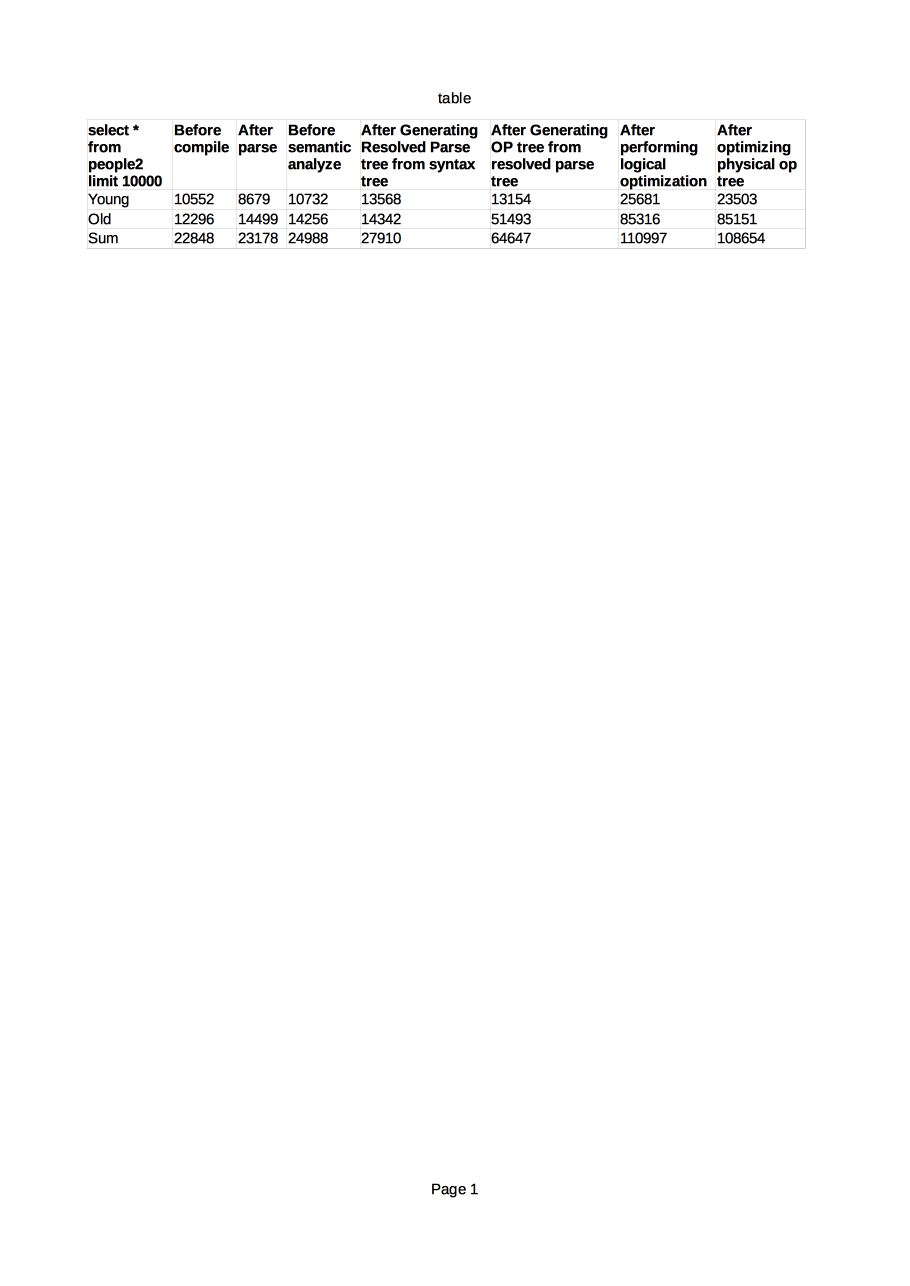
\includegraphics[width=150mm, keepaspectratio]{figures/parse_output.png}
	\centering
	\caption{Sample output of the parsing}
\end{figure}


\subsection{How HiveServer2 uses memory}
I have the code to measure the memory of Hive and get a general picture of the usage at certain phases. With this, I am able to get a better understanding when and why memory goes high. I would like to get an answer to these questions: How does the number of joins increase the memory? Which type of query generates a lot of memory usage: union, group by? If we increase the number of partitions, how it affects the heap size? In this section, these questions will be answered.

The first step is to create a managed table where I will run my queries in the future. Hive faces memory problems when we have a highly partitioned table. I decided that for the first run, 20 000 partitions will be enough. 

The second step was to create queries which will be submitted to Hive. The first question was how the number of joins affects memory? To answer it, I have created queries with an increasing number of joins included. I used self-joins and only increased the number to three. The pattern was clear for only four measures: a simple select query without join operator, and queries with one, two and three. From the output of my parsed CSV file, I generated the following chart that shows the memory increase.

\begin{figure}[H]
	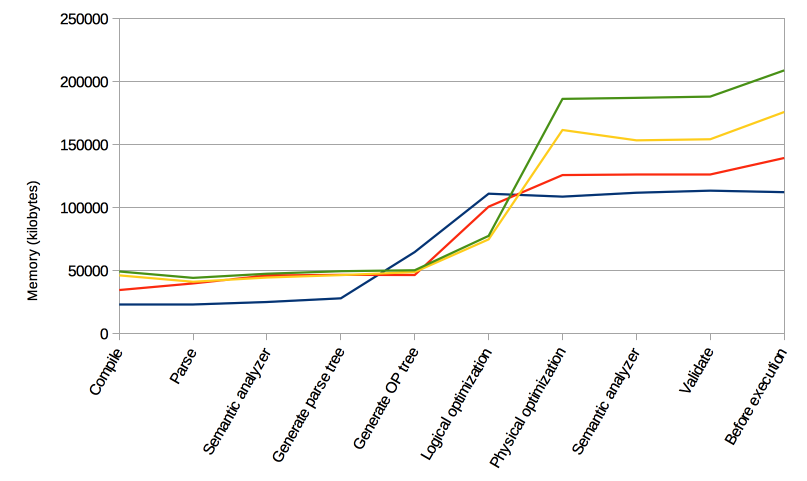
\includegraphics[width=150mm, keepaspectratio]{figures/hs2_joins_memory.png}
	\centering
	\caption{Heap size with increasing number of joins}
\end{figure}

\noindent Queries run with their color in the chart:
\begin{itemize}
	\item select * from tablename (\textcolor{blue}{\rule{2 cm}{2pt} })
	\item select * from tablename t1 join tablename t2 on t1.id=t2.id (\textcolor{orange}{\rule{2 cm}{2pt} })
	\item select * from tablename t1 join tablename t2 on t1.id=t2.id join tablename t3 on t2.id=t3.id (\textcolor{yellow}{\rule{2 cm}{2pt} })
	\item select * from tablename t1 join tablename t2 on t1.id=t2.id join tablename t3 on t2.id=t3.id join tablename t4 on t3.id=t4.id (\textcolor{green}{\rule{2 cm}{2pt} })
\end{itemize}

We can see that the memory change caused by the number of join operators is negligible, only around 20 Megabytes per join. The results were as expected: the memory increased significantly when HiveServer2 connected to the MetaStore and asked for metadata. During physical optimization, Hive loaded metadata to memory including partition metadata. In a highly partitioned table, this size is notable. Although real queries submitted to Hive by users are much more complicated and contains multiple tables, the model will be quite similar: heap memory will rise when metadata is loaded.

I also wanted to see the memory effects of \textit{group by} and  \textit{union all} operations. I ran 5 more queries including these but did not find anything notable. The pattern remained the same: see the chart below. 

\begin{figure}[H]
	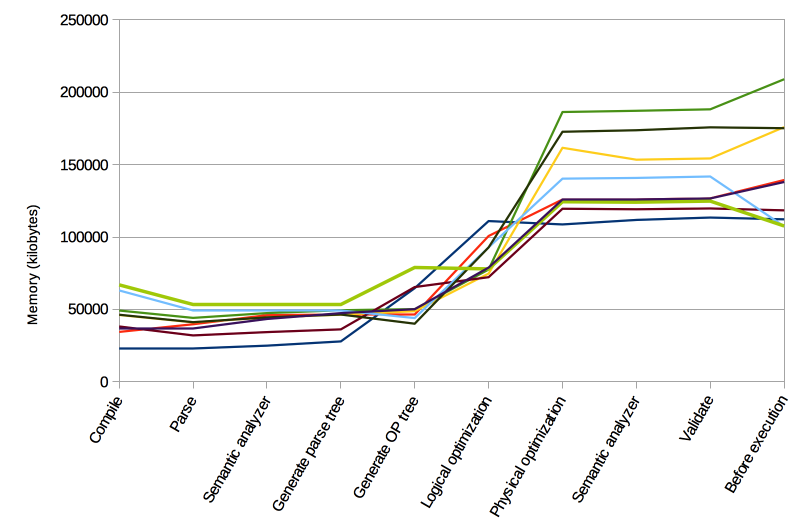
\includegraphics[width=150mm, keepaspectratio]{figures/hs2_memory.png}
	\centering
	\caption{Heap size when running various type of queries}
\end{figure}

I came to the conclusion that for a single connection to HiveServer2, the most important factor that increases heap size is the number of partitions in tables, so I decided to continue my investigation in that area. 

\subsection{Memory consumption of partitions}
A well-known issue in Hive is, if we have a highly partitioned table, the memory goes really high in HiveServer2. As a first step, I wanted to recreate the issue. I created tables with an increasing number of partitions: 200, 2000, 5000, 20000 and 100000 partitions. For each table, I executed the same query which contains a simple select with a self-join. During this, I measured the memory and created a heap dump after the semantic analyzer phase of the compilation. At this stage, the partitions are already loaded so I can analyze how much these objects exactly reserve. To get this information, I analyzed the heap dumps with VisualVM and filtered for the Partition objects. The pattern we can observe was as expected, but I the size of the heap reserved by these objects were smaller than I previously anticipated.

\noindent From the heap dumps I have found that mainly three kind of objects reserve the memory due to partitions, so I will focus on these objects: 
\begin{enumerate}
	\item hive.ql.metadata.Partitions
	\item hive.metastore.api.Partition
	\item hive.ql.plan.PartitionDesc
\end{enumerate}

\begin{table}[H]
	\begin{tabular}{|l|l|l|l|l|}
		\hline
		& \textbf{\begin{tabular}[c]{@{}l@{}}ql.metadata.\\ Partitions\end{tabular}} & \textbf{\begin{tabular}[c]{@{}l@{}}metastore.api.\\ Partition\end{tabular}} & \textbf{\begin{tabular}[c]{@{}l@{}}ql.plan.\\ PartitionDesc\end{tabular}} & \textbf{Sum} \\ \hline
		\textbf{200 partitions}    & 300 Kb                                                                     & 288 Kb                                                                      & 108 Kb                                                                    & 696 Kb       \\ \hline
		\textbf{2000 partitions}   & 3057 Kb                                                                    & 2946 Kb                                                                     & 1110 Kb                                                                   & 7113 Kb      \\ \hline
		\textbf{5000 partitions}   & 7988 Kb                                                                    & 7709 Kb                                                                     & 2793 Kb                                                                   & 18490 Kb     \\ \hline
		\textbf{20000 partitions}  & 29999 Kb                                                                   & 28879 Kb                                                                    & 3173 Kb                                                                   & 62051 Kb     \\ \hline
		\textbf{100000 partitions} & 165002 Kb                                                                  & 158841 Kb                                                                   & 60531 Kb                                                                  & 384374 Kb    \\ \hline
	\end{tabular}
\caption{Memory of partitions}
\end{table}

\begin{figure}[H]
	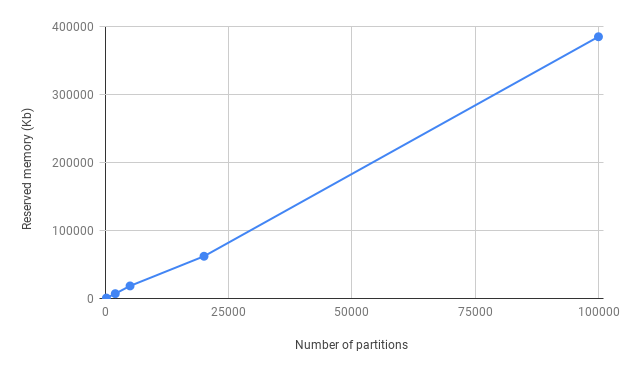
\includegraphics[width=150mm, keepaspectratio]{figures/partitions_chart.png}
	\centering
	\caption{Reserved memory by partitions}
\end{figure}

As we see, for 100.000 partitions the reserved memory is aroung 385 Megabytes. Before taking the samples, I expected higher memory consumption. However, with a little investigation I found that the memory waste around partitions was already somewhat decreased \cite{hive-partitions}. PartitionDesc objects has a java.util.Properties field. These Properties fields in the PartitionDesc most often are the same. Interning these saves a big amount of memory. In a later section, I will write more about the interning solution because it gave me an idea to fix another memory related issue.

However the memory reserved by partitions is still high enough, so I decided to take a look at the heap dumps and try to find wastes or problems that affects memory.

\subsection{Where does the memory go?}
I analyzed the heap dump generated after the semantic analyzer phase when self-joining a table with 100000 partitions. It showed an interesting fact: 47.1\% (~853 Megabytes) of retained memory is reserved by Strings. Retained means, that if the Garbage Collector frees them, we win that amount of memory. 

\begin{figure}[H]
	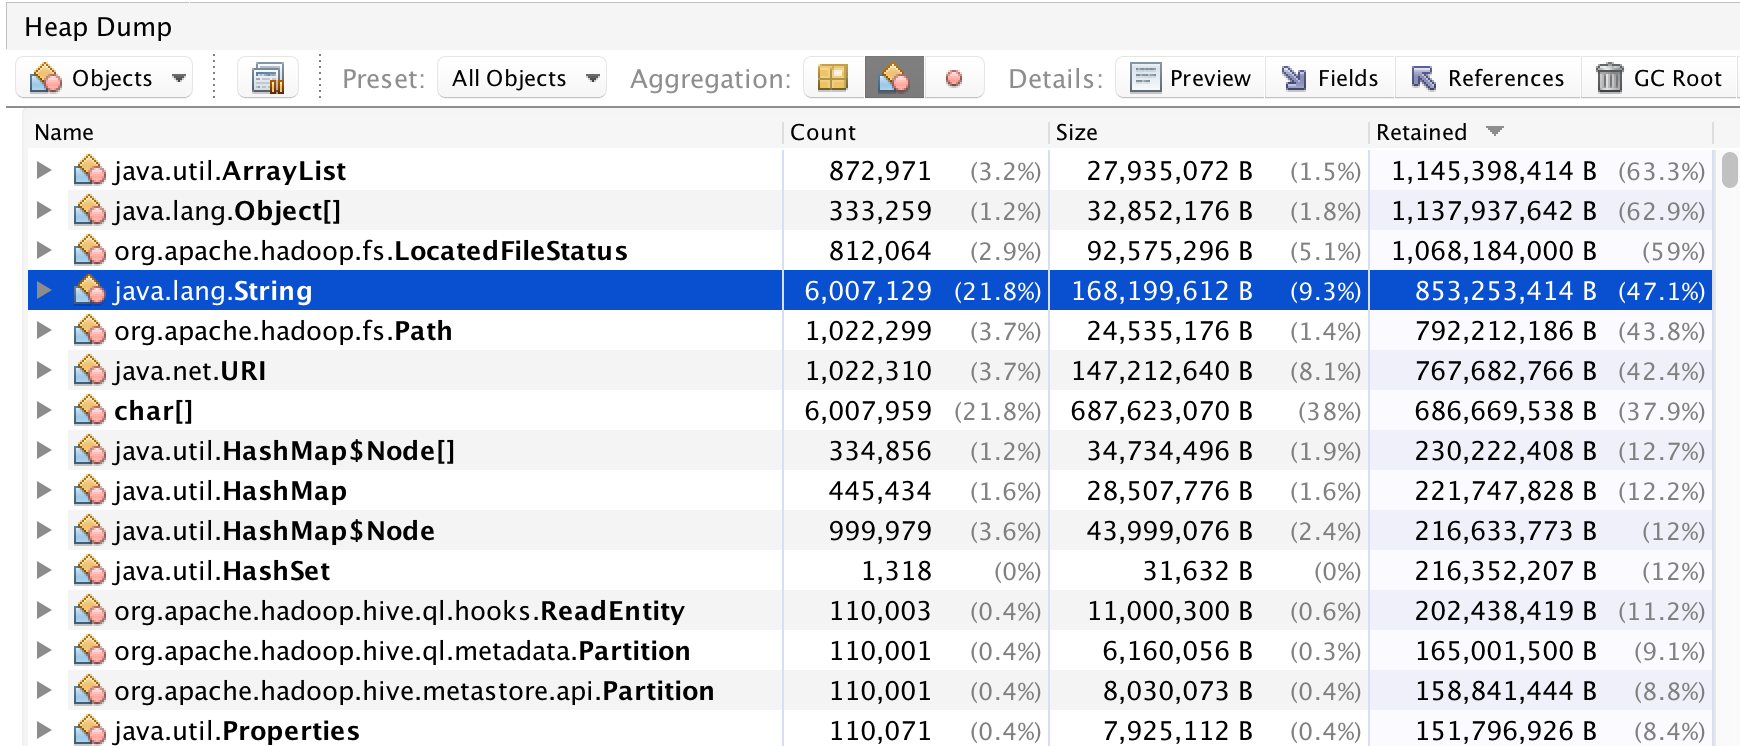
\includegraphics[width=150mm, keepaspectratio]{figures/string_memory.png}
	\centering
	\caption{Memory reserved by Strings}
\end{figure}

We also see in the above image that \textit{hadoop.fs.Path} objects reserve 792 Megabytes. It seems too much considering that we only speak about the location of a file in the filesystem. As a next step, I looked inside the Path objects to see if this is a waste or not.

\subsubsection{Memory waste in HDFS Path}
\begin{figure}[H]
	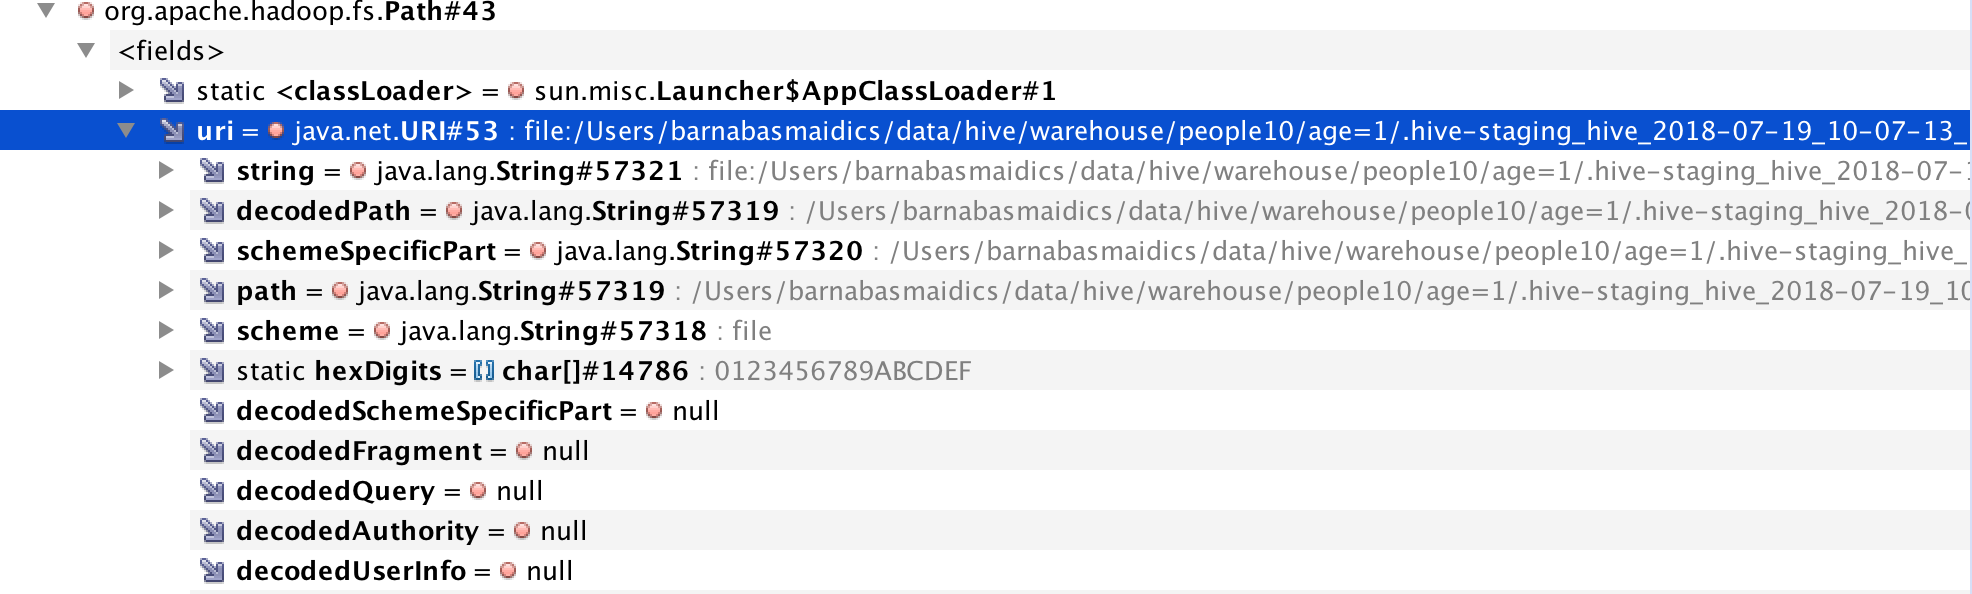
\includegraphics[width=150mm, keepaspectratio]{figures/path_memory.png}
	\centering
	\caption{Inside of a Path}
\end{figure}

In Path objects, we store the location in a \textit{java.net.URI} object. Its internal representation seems really wasteful. As we see, URI stores a path in 3 different Strings. The Strings are almost the same: for example the string field inside the URI contains the scheme, the path field does not, and this is the only difference \etc. We can ask ourselves: is it really necessary?

To determine this we need to inspect the Path.java source code. URIs are always created the same way: we pass four String parameters to the constructor of the URI class: scheme, authority, path, and fragment. In the code below the null parameter represents the query part of a URI. Passing null means that we do not need that value.

\begin{lstlisting}
	newUri = new URI(scheme, authority , path, null, fragment);
\end{lstlisting}

To summarize, the internal representation of the URIs clearly seems like a waste of memory. So I started to think of an alternative solution to replace these URI objects and save around 66\% of memory for each Path. 

\chapter{Fixing memory waste of URIs - HDFS-13752}
The duplication comes from the \textit{java.net.URI} objects so the first thing that came to my mind was to replace this with a more memory efficient implementation in the Path.java class. As a first approach, I created a Jira ticket in the corresponding Apache site to report the issue \cite{hdfs-path}. 

The community agreed that the way URIs store these paths is a waste, and could be stored more efficiently. However, many other classes use these URIs. The Path class has a public \textit{toURI} function which returns the URI representation of the path. Obviously, this cannot be removed because others are depending on it. I found three possible solutions to get rid of this memory overhead.

\begin{itemize}
	\item Keep the URI field with only having a WeakReference to it, and store the 4 parts of the Path in seperate fields
	\item Keep the URI field with only having a SoftReference to it, and store the 4 parts of the Path in seperate fields
	\item Remove the URI field completely and store those parts of the URI that we really use in separate Strings
\end{itemize}
\section{Solution ideas}
\subsection{Solution 1: WeakReference}
A WeakReferenced object works in a way, that if the object is only weakly reachable (its only reference is a WeakReference), it will not prevent the object to be garbage collected. We would have a WeakReference to the URI and when the GC runs it can collect the URIs if iwe do not have a strong reference to it. 

When someone wants to get the URI representation of the path and calls the \textit{toURI} function, we need to check if the URI exists through the WeakReference or not. If it exists we can just get it because we have a WeakReference to it. If it does not, we need to recreate the URI from its parts. 

\subsection{Solution 2: SoftReference}
Using SoftReference would be a more conservative solution. If the Garbage Collector finds an object that is only softly reachable, it does not dump the object instantly. An object with a SoftReference will only be collected at memory demand. This way before an Out Of Memory error is thrown, the GC can free all URIs. If the GC collected the URI we would do the same as mentioned before: recreate the URI from the stored parts when needed. 

\subsection{Solution 3: On demand URI creating}
A possible solution is to remove the URI completely and only keep 4 parts of the Path which are used: scheme, authority, path and fragment. This way we can immediately win around 66\% of memory. The only drawback is that we always have to recreate the URI every time the toURI method is called and this might be expensive CPU-wise.

\begin{figure}[H]
	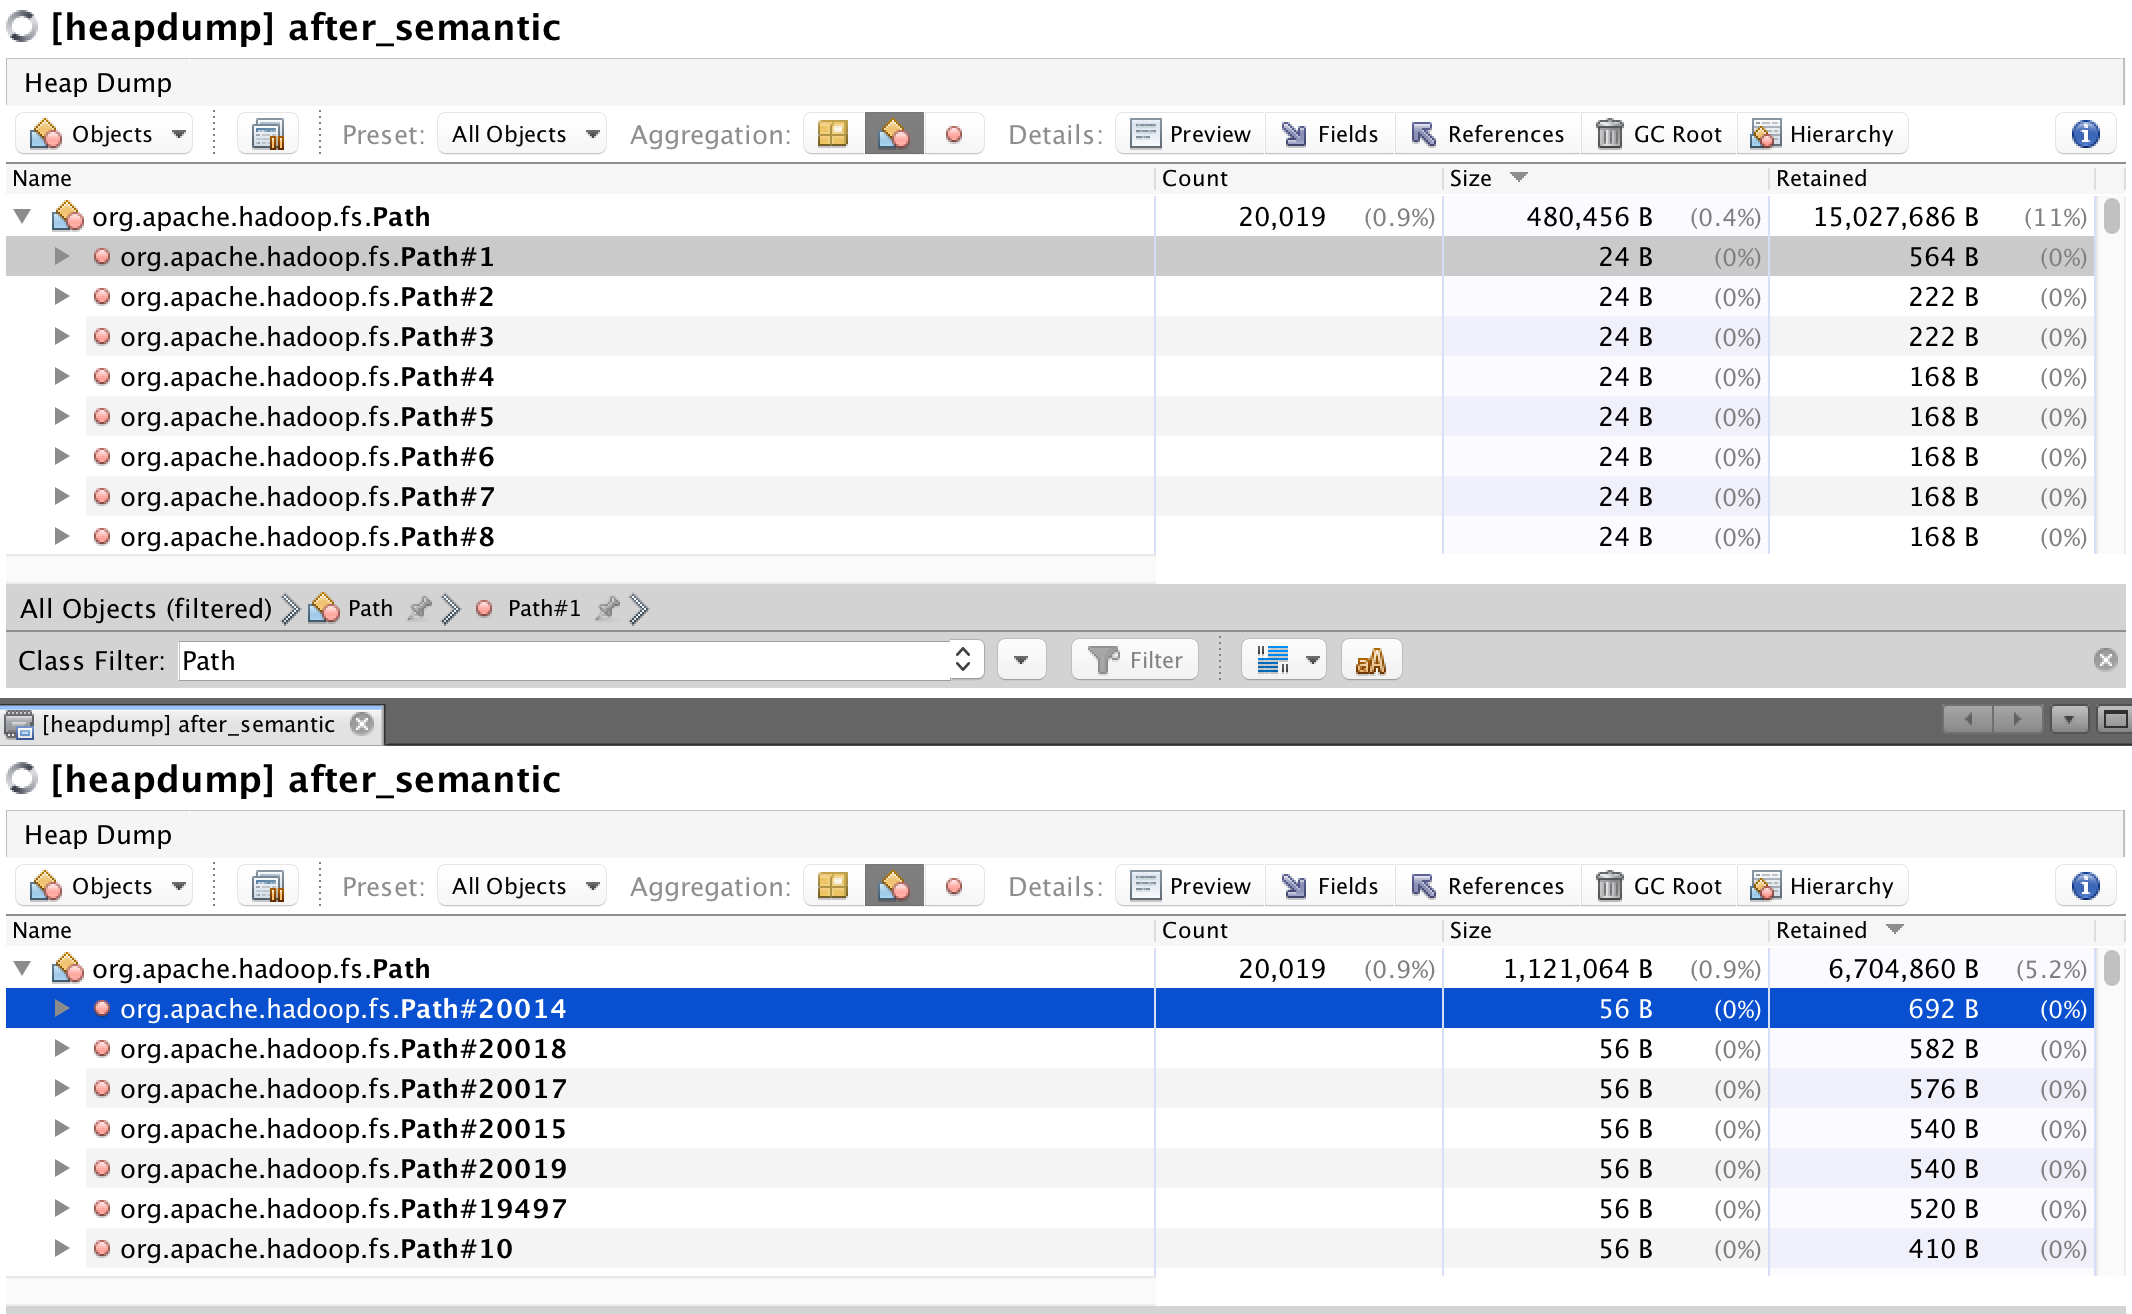
\includegraphics[width=150mm, keepaspectratio]{figures/path_before_after.png}
	\centering
	\caption{Memory save of Paths}
\end{figure}

\subsection{Conclusion}
For the second thought, I realized that using WeakReference would not be the best decision. It would almost be the same as creating the URI on demand, since whenever the GC runs, it will collect the URIs immediately and when toURI is called we would have to recreate it anyway. The only way to decide which solution might be the best is to measure the performance of both approach. 

I also analyzed the code base of Hadoop to see how \textit{Path.toUri} method is usually used. Most often we just want to ask for certain parts of the Path object and not really using the URI itself. For example: \textit{pathObject.toUri().getPath()} to get the path or \textit{pathObject.toUri().getScheme()} to get the scheme. Considering only this, solution 3 would be the most effective, since we are able to get the path/scheme/authority or fragment directly from the Path object and we do not need to first transform it to an URI and than ask for the value we need. 

\section{A simple performance test for toURI}
I created a really simple test, to decide which solution would solve the issue without a significant CPU overhead. 

I tested the CPU usage of the toUri() method, analyzing the different solutions: I created 1.000.000 Path objects (of course this is not a real use case, but it can be a good estimation as the first approach). See the results in the table below (3. row). I’ve also measured the memory effects of the changes. 

\noindent The code I used for testing:
\begin{lstlisting}
long startTime = System.nanoTime();
for(int i=0; i<1000000; i++){
	paths[i].toUri().getPath();
}
long estimatedTime = System.nanoTime() - startTime;
\end{lstlisting}

\begin{table}[H]
	\begin{tabular}{|l|l|l|l|}
		\hline
		& \textbf{Original} & \textbf{\begin{tabular}[c]{@{}l@{}}SoftReference \\ (solution 2)\end{tabular}} & \textbf{\begin{tabular}[c]{@{}l@{}}New URI \\ (solution 3)\end{tabular}} \\ \hline
		\textbf{Memory of the Paths}     & 608 MB            & 664 MB                                                                         & 238 MB                                                                   \\ \hline
		\textbf{Time of the toURI calls} & 0.12973 s         & 0.04142 s                                                                      & 1.29133 s                                                                \\ \hline
	\end{tabular}
\centering
\caption{Results of the test}
\end{table}

The results showed that using SoftReference has a bit of memory overhead because apart from the URI itself, we need to store the SoftReferences which require heap space as well. Thus, it would only be a save if the heap is almost full, other than that we it would reserve even more memory. The time of toURI calls might be deceptive. Calling \textit{toURI} method only once is slower than with the original solution and we do not use the method as in the example above. 

Looking into the results of the third possible solution, the benefits are clear memory-wise. However, the time of the toURI calls do not look so promising. The CPU time is almost 10x bigger than with the original approach. But if we take into account other factors, not just the plain CPU time, the overhead might not be that big. If the memory of the paths are reduced, the GC can work much faster, so smaller GC pauses will occur. Also, these Path objects passed through the interface of Hadoop in both direction. For example, NameNode gives the location of files in the format of Paths and Hive passes these objects to Hadoop as well. Considering these, my change would be possibly beneficial for transfering data through the network: Passing objects which are smaller is obviously faster. 

An additional factor that should be considered is that if we remove the \textit{toUri} call whenever we want to get the values of path, scheme, authority or fragment, we can improve the performance of the original solution, since we can get those directly. Instead of \textit{Path.toUri().getPath() } we can just say \textit{Path.getPath()}.

To test this theory, I created a simple test. The times of 1.000.000 toUri().getPath() calls:
\begin{itemize}
	\item Original: 0.143235527 s
	\item Solution 3 if Path.toUri().getPath() staying: 1.316882214 s
	\item Solution 3 with only Path.getPath(): 0.004373138 s
\end{itemize}

With the results of my test, I decided to choose solution 3, which may be the simplest fix: remove the URI field completely and if someone needs it, create on demand from the path, scheme, authority and fragment parts.

\section{Performance test on a cluster}
As a next step, I configured a cluster to see if my change would affect CPU significantly. The cluster I created had 4 nodes and only HDFS, YARN and HIVE were installed. I generated the below HDFS directory structure to test the performance of my fix. The "perftest" directory contains 100 folders, each contains 1000 other folders with one txt file. The code I used for testing can be found in the Jira ticket I reported \cite{hdfs-path} (HDFS-13752.003.patch).

\begin{figure}[H]
	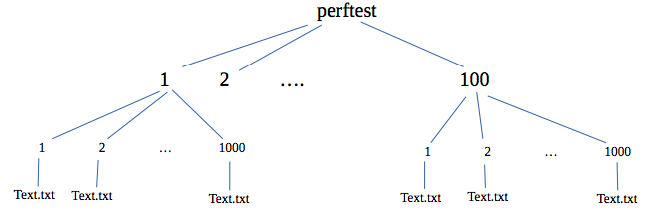
\includegraphics[width=125mm, keepaspectratio]{figures/directory_structure.png}
	\centering
	\caption{Directory structure of the test}
\end{figure}

For the tests, I used FileSystem shell to interact with the HDFS directly. I choosed one shorter and one longer running operation for measuring the CPU time. The values in the tables are in millisecond.

\subsection{Listing files recursively}
The command used:  \textit{hdfs dfs -ls -R /user/perftest}

\begin{table}[H]
	\begin{tabular}{|l|l|l|l|l|l|l|}
		\hline
		& \textbf{M1} & \textbf{M2} & \textbf{M3} & \textbf{M4} & \textbf{M5} & \textbf{Avg} \\ \hline
		\textbf{Original} & 42651    & 38136    & 40183    & 41749    & 36963    & 39936     \\ \hline
		\textbf{New URI}  & 41762    & 39219    & 38800    & 37315    & 37719    & 38963     \\ \hline
	\end{tabular}
\centering
\caption{CPU time of a recursive listing}
\end{table}
\subsection{Changing the replication factor of a file}
The command used:  \textit{hdfs dfs -setrep -w 3 /user/perftest}

\begin{table}[H]
	\begin{tabular}{|l|l|l|l|l|l|l|}
		\hline
		& \textbf{M1} & \textbf{M2} & \textbf{M3} & \textbf{M4} & \textbf{M5} & \textbf{Avg} \\ \hline
		\textbf{Original} & 172240      & 179050      & 193963      & 189105      & 171446      & 181161       \\ \hline
		\textbf{New URI}  & 185523      & 169111      & 171326      & 171451      & 170389      & 173560       \\ \hline
	\end{tabular}
\centering
\caption{CPU time of a replication factor changing}
\end{table}

\subsection{Analyzing the results}
Seeing the results I think there is no big performance difference. The new solution is even a little bit faster. A possible explanation for this is that I removed several \textit{toUri()} calls inside the Path class, because we store the Path, Scheme, Authority and Fragment in the Path object. These can also be done outside of the Path class. Another explanation can the network improvement mentioned before or even the decrease of the GC pauses. Or it may only be just the inaccuracy of the measurement.

\section{Effects of the change in Path}
After publishing the results to the Apache HDFS Jira, I tried to investigate if the change would be really beneficial. These Path objects can be found in every component that uses Hadoop, like Hive, Impala, HBase \etc and used widely everywhere in the code. As a consequence of this, a little CPU overhead can even cause a big performance loss so the patch needs to be tested throughly. 

If this little change has some possibility to decrease the performance significantly, would it really benefit the components? I did an investigation to see if this issue is real and what would it fixed. Based on the results, my answer is: yes. The following issues was partly or entirely caused by the size of memory these Path objects reserve, so reducing the size with 66\% may solve or help these problems.

\subsection{Hive MetaStore OOM}
During my investigation I found a HMS memory issue in production use of Hive. The MetaStore server crashed due to an Out Of Memory error. The following heap dump was created before the OOM. Here 9.743 Gigabytes of memory was used by \textit{fs.Path} objects.

\begin{figure}[H]
	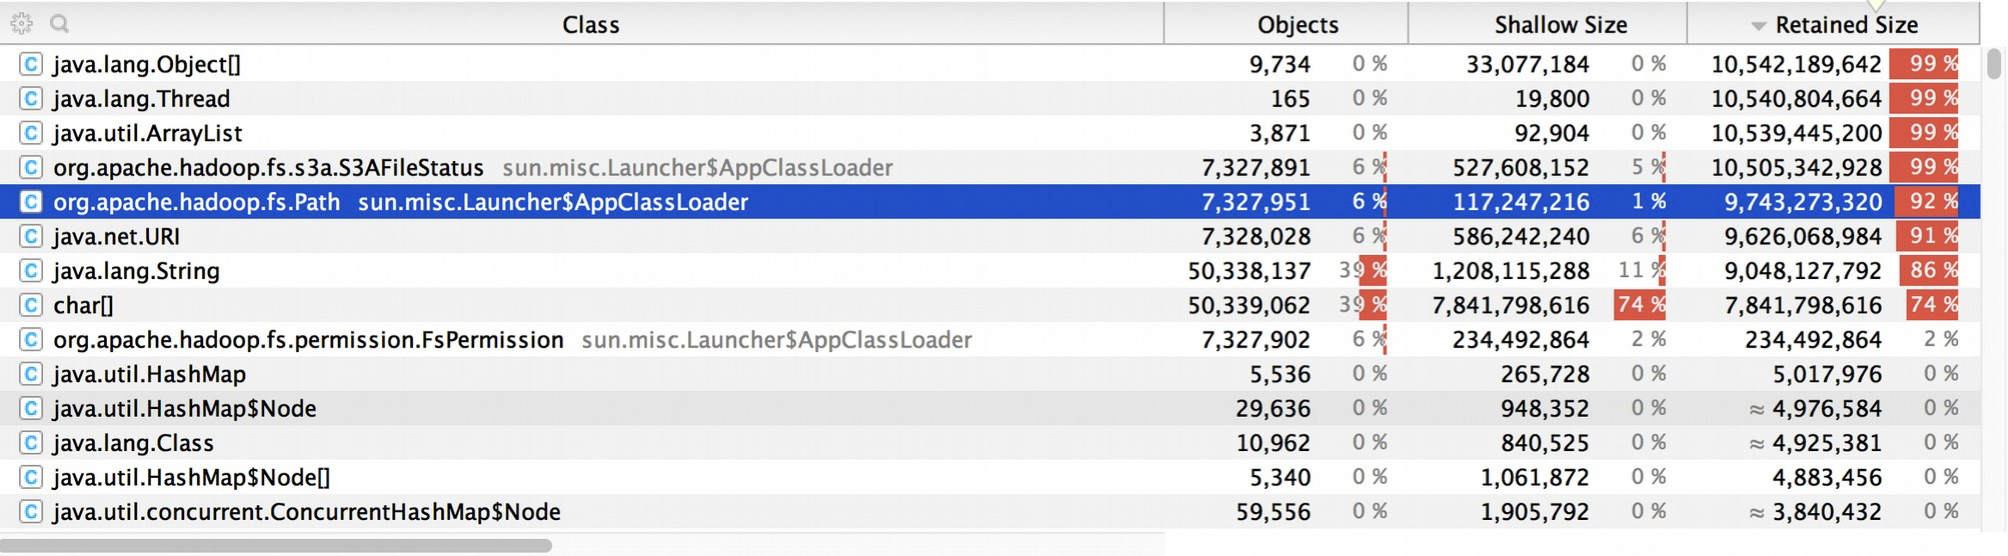
\includegraphics[width=150mm, keepaspectratio]{figures/hms_heapdump.png}
	\centering
	\caption{HMS heap dump before OOM}
\end{figure}

\subsection{Hive on Spark memory issue}
Stress testing of HoS (Hive with Spark execution engine) has revealed that we have memory issues when running with a high value of \textit{spark.executor.cores}. The overhead is mainly introduced by loading multiple copies of HiveConf (Hive configuration object) and there is a significant overhead when loading lots of Path objects too. In the next chapter I will focus on the multiple HiveConf issue as well.

\subsection{"Small files problem" in HiveServer2}
HS2 has a so called "small files problem". Something like \textit{create external table} with lots of small files in the  HDFS directory of the table causes HiveServer2 to load the HDFS paths of the files into memory. If we have millions of small files (which is not that rare), these paths can use Gigabytes of heap memory. Hive does a \textit{listFiles} that returns all the Paths, to determine file permissions \etc. So create table hangs and other queries wait a LOT.

\subsection{Apache Impala's solution for the problem}
Apache Impala also faced problems caused by the size of memory used by the Paths. Impala is a query engine on top of Hadoop, similar to Hive. They already solved this problem on their side. Impala has a \textit{HdfsPartitionLocationCompressor.java} class which they use to solve exactly this problem. I also thought of the idea to solve the issue in Hive, however for a long term, it may not be the most desirable strategy. Hive would have to always convert the Paths whenever it passes them to Hadoop (Impala does this). I think if the problem can be solved in  Hadoop - where it comes from - without a performance overhead, it should be done there. My task is to give the community a proof that CPU overhead will not happen because of the memory fix. 

\section{Benchmarking on a data center cluster}
The patch would effect every part of Hadoop, so a thorough benchmark is needed. The performance tests run on a data center cluster with Hadoop 3.0.0 for more than a month. From 13 September to 25 September without my patch, from 26 September to 19 October with my patch. The following charts will show the results for some test cases. On these diagrams, the values before the red line are without my patch and after the red line are the values including my patch. I created several diagrams to show the full result to the community. I will only include a part of them here, the full document can be found on the Jira ticket (HDFSbenchmark.pdf) \cite{hdfs-path}.

\noindent Parameters of the benchmarks: 
\begin{itemize}
	\setlength{\itemsep}{1pt}
	\item Number of worker nodes: 7
	\item Dataset size per node: 1000 GB
	\item Number of mappers per node: 80
	\item Filesize for TestDFSIO: 16 GB
	\item Number of files for NNBenchmark: 50000
\end{itemize}

\subsection{TeraSort benchmark}
"TeraSort reads the input data and uses MapReduce to sort them." \cite{terasort}

\begin{figure}[H]
	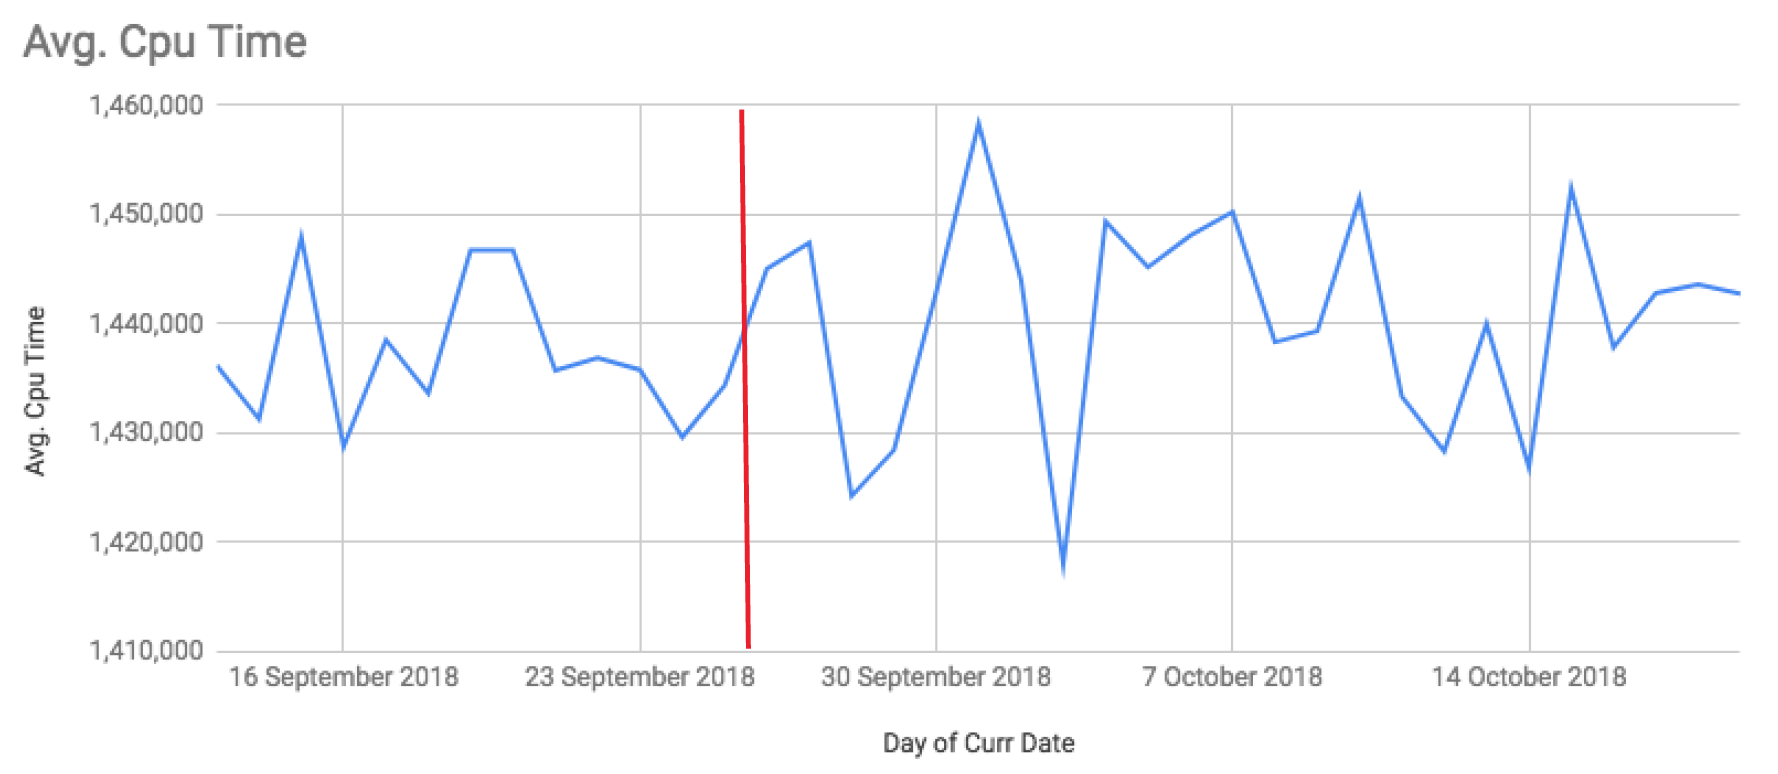
\includegraphics[width=125mm, keepaspectratio]{figures/terasort_cpu.png}
	\centering
	\caption{TeraSort Average CPU time}
\end{figure}
\begin{figure}[H]
	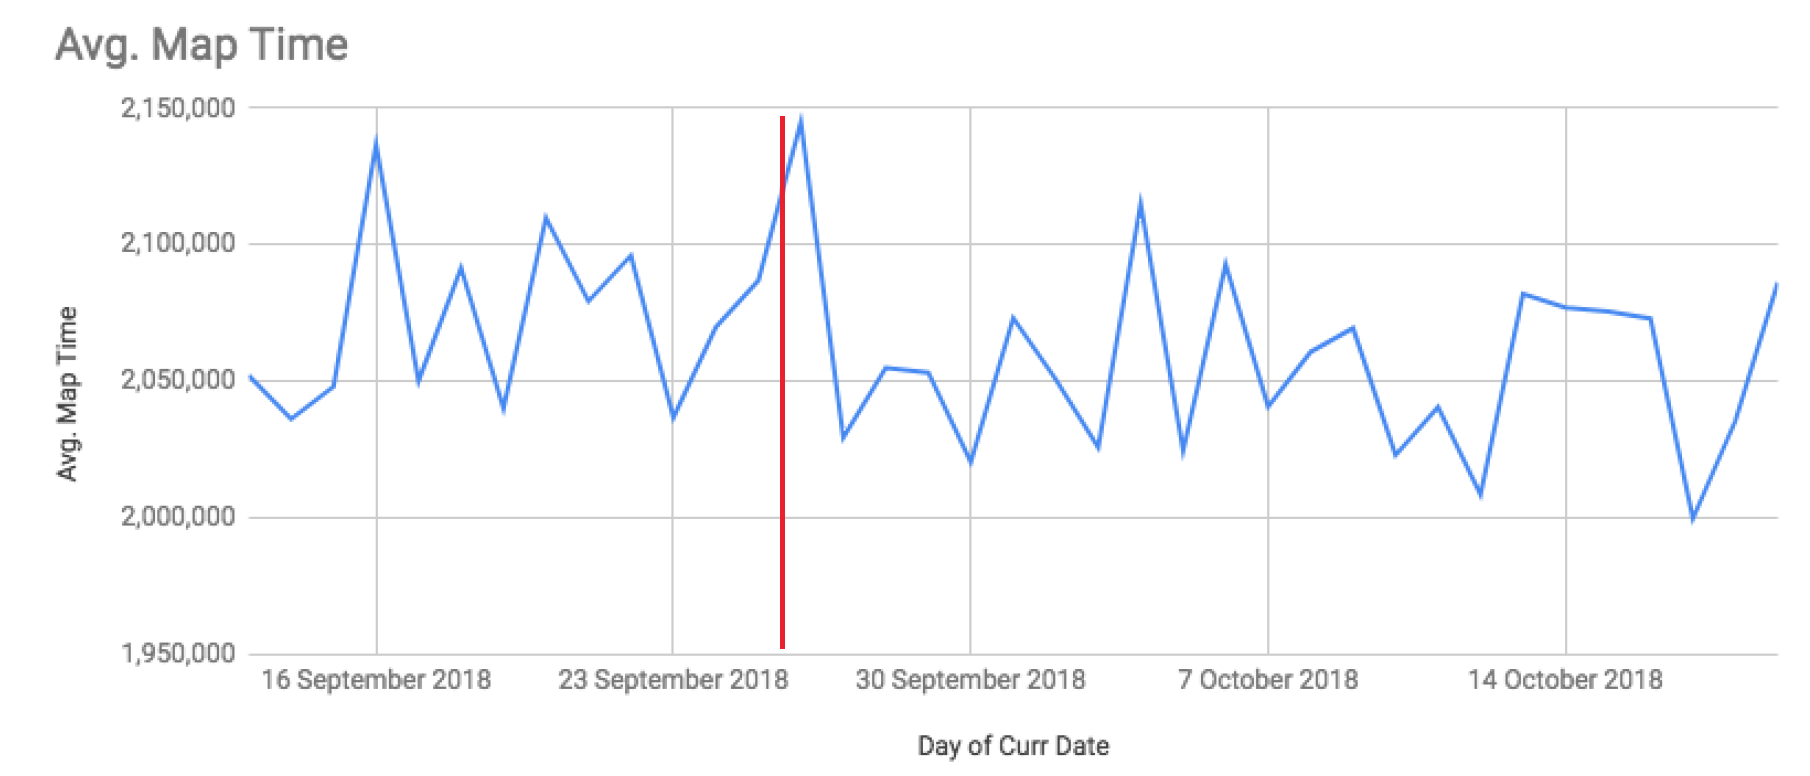
\includegraphics[width=125mm, keepaspectratio]{figures/terasort_map.png}
	\centering
	\caption{TeraSort Map time}
\end{figure}
\subsection{TeraValidate benchmark}
"TeraValidate validates the sorted output to ensure that the keys are sorted within each file. If anything is wrong with the sorted output, the output of this reducer reports the problem." \cite{terasort}

\begin{figure}[H]
	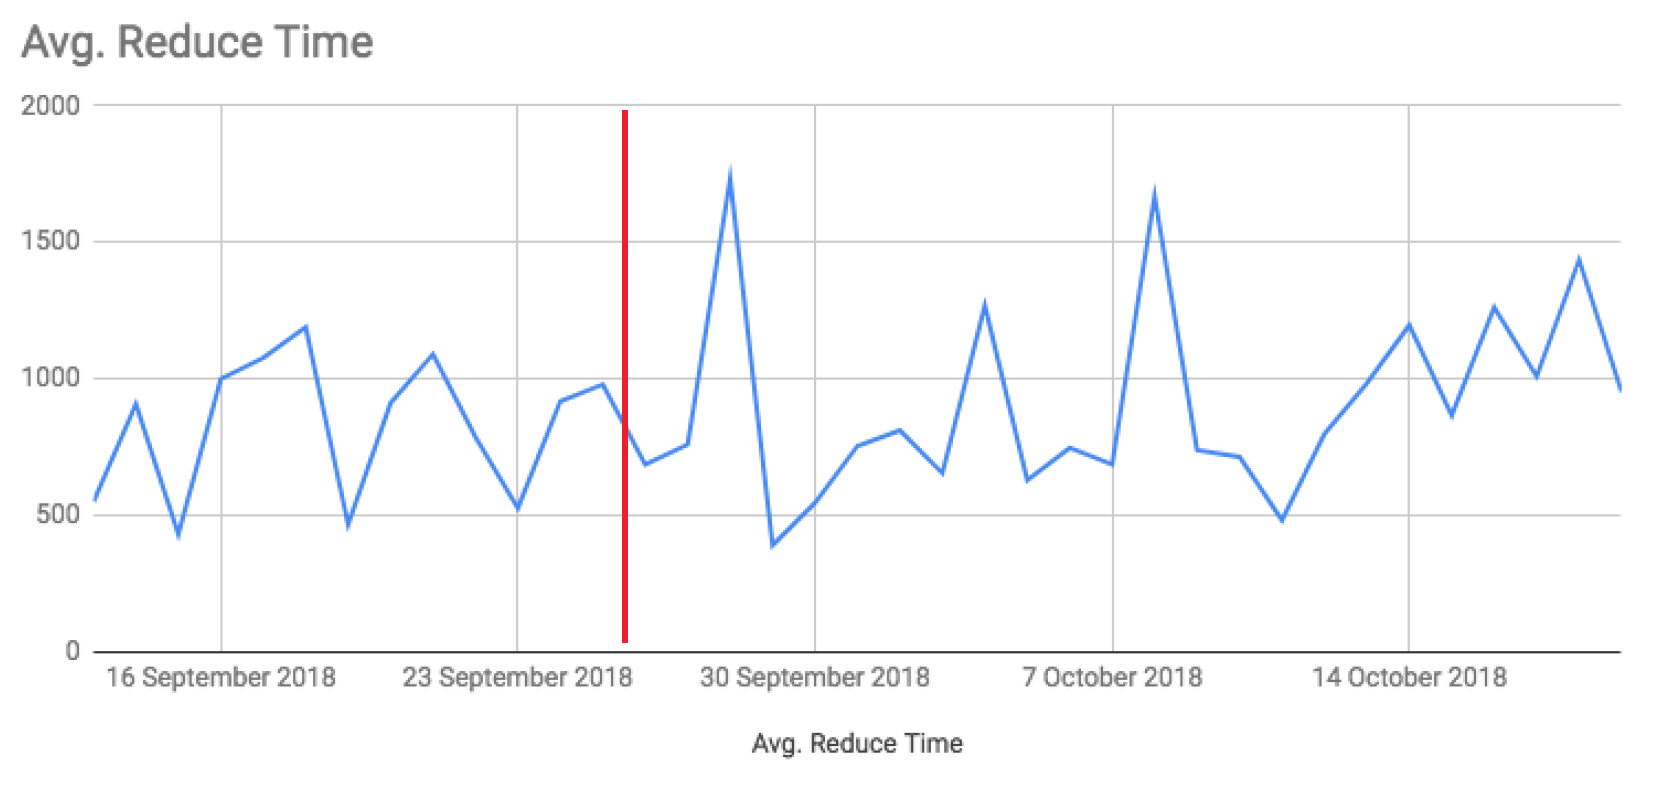
\includegraphics[width=125mm, keepaspectratio]{figures/teravalidate_job.png}
	\centering
	\caption{TeraValidate Job time}
\end{figure}
\begin{figure}[H]
	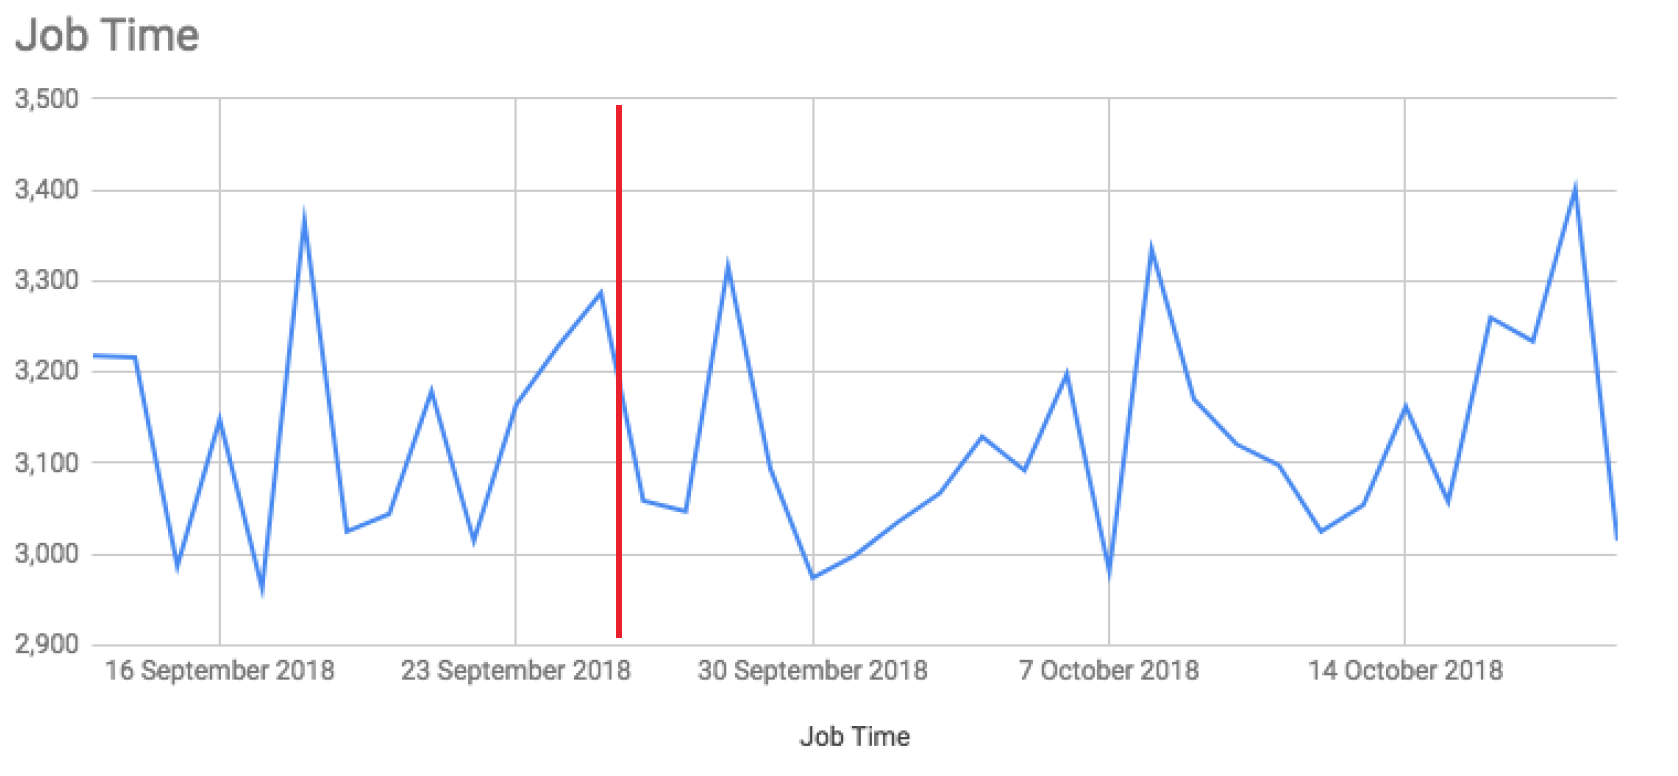
\includegraphics[width=125mm, keepaspectratio]{figures/teravalidate_reduce.png}
	\centering
	\caption{TeraValidate Reduce time}
\end{figure}

\subsection{TestDFSIO}
TestDFSIO is a benchmark for measuring the capacity of HDFS for reading and writing data. It is helpful to discover performance bottlenecks.

\begin{figure}[H]
	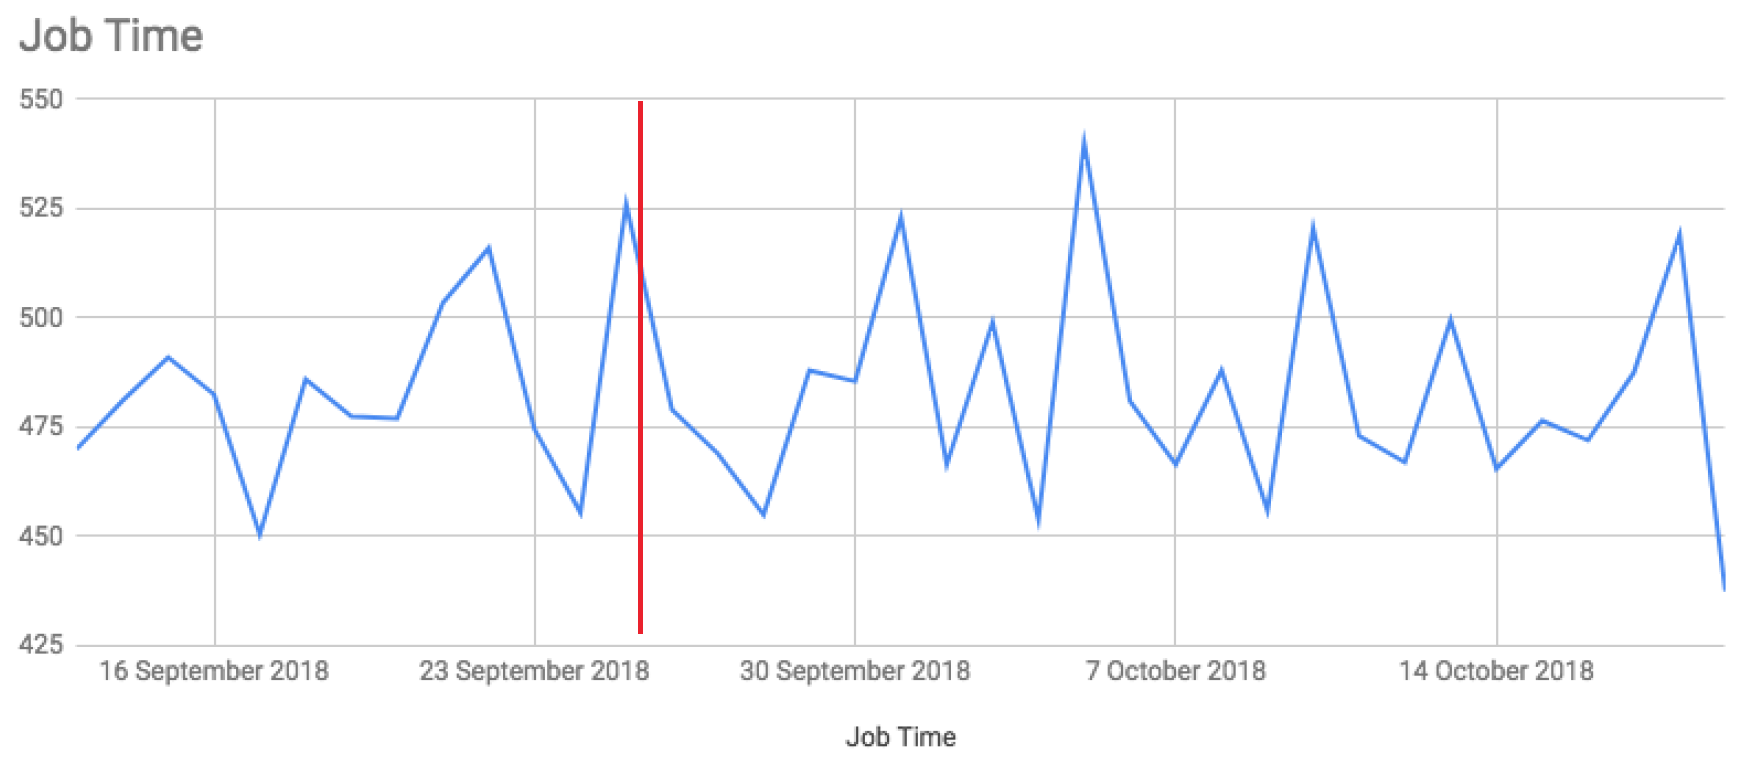
\includegraphics[width=125mm, keepaspectratio]{figures/dfsio_job.png}
	\centering
	\caption{TestDFSIO Job time}
\end{figure}

\subsection{NNBench - NameNode stress test}
This benchmark generates a lot of HDFS requests for putting a high HDFS management stress on the NameNode. The benchmark can create, read, rename and delete files on HDFS.

\begin{figure}[H]
	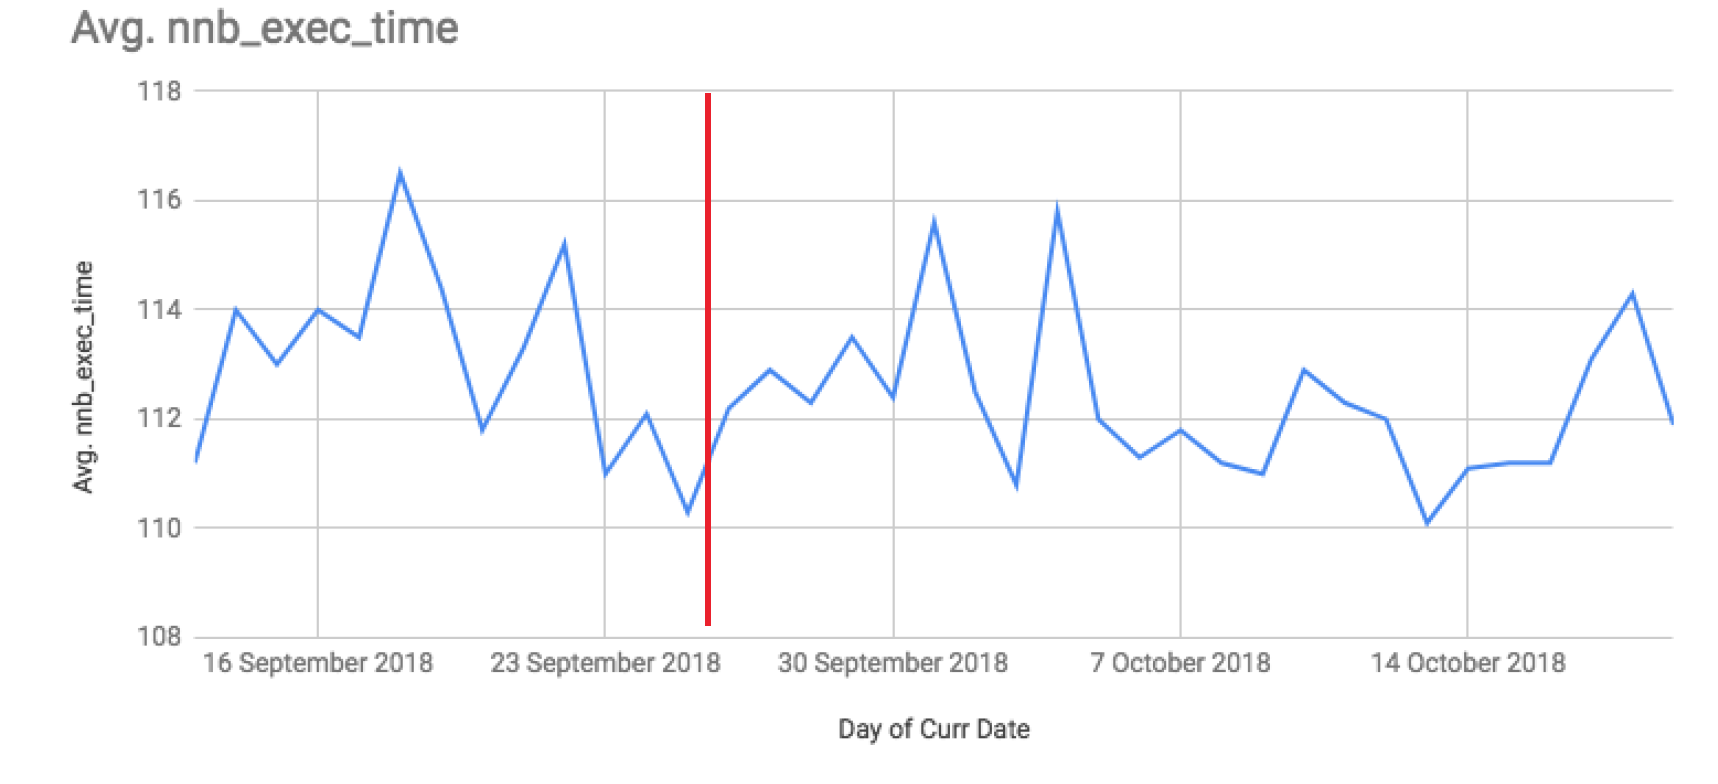
\includegraphics[width=125mm, keepaspectratio]{figures/nn_exec.png}
	\centering
	\caption{NameNode execution time of open\_read operation}
\end{figure}
\begin{figure}[H]
	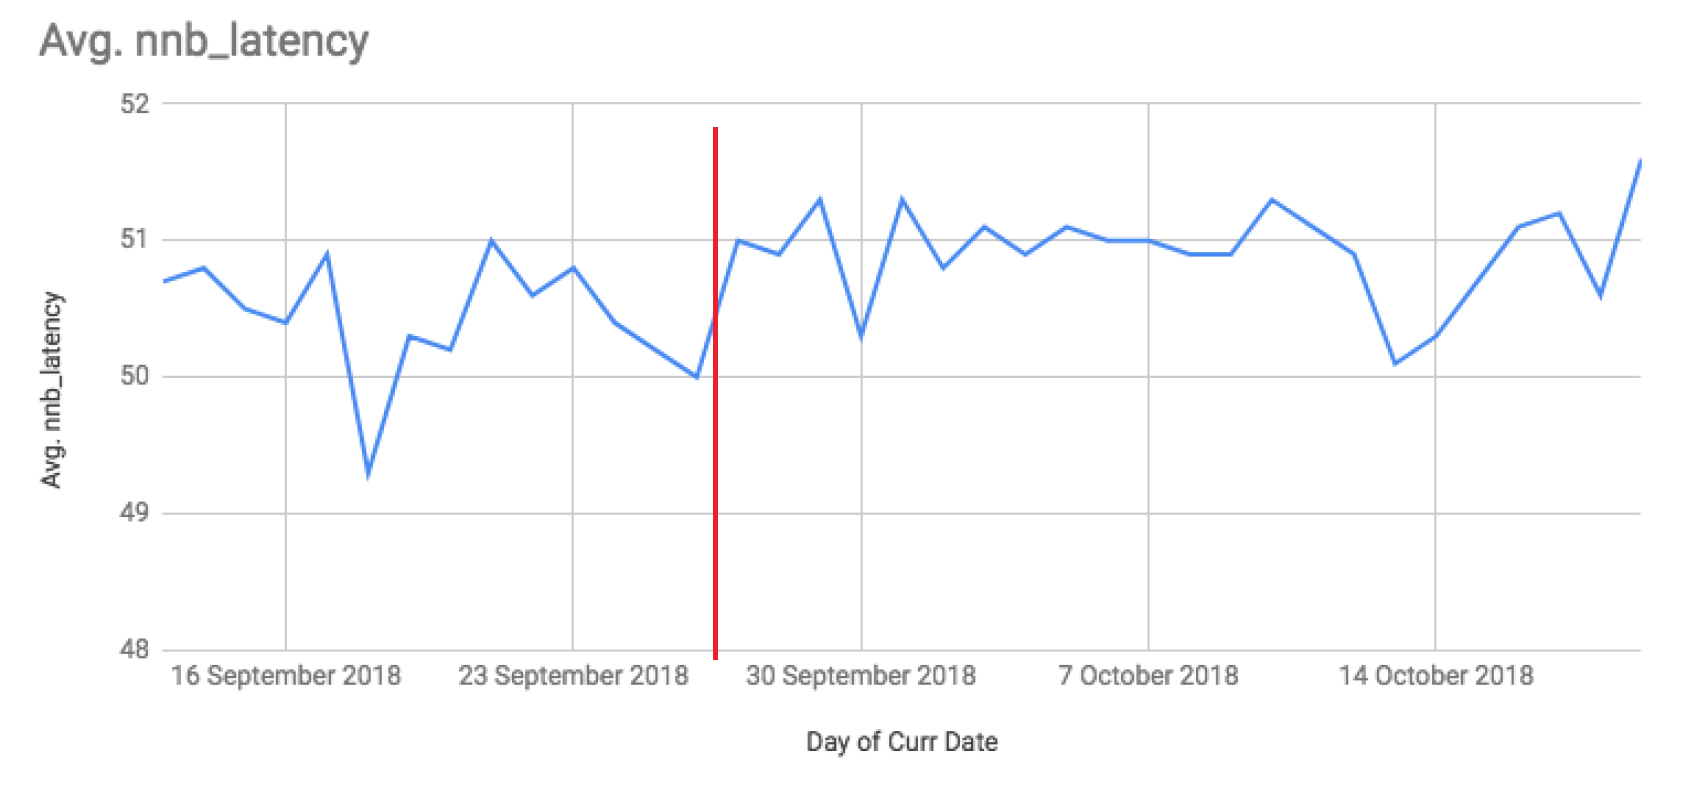
\includegraphics[width=125mm, keepaspectratio]{figures/nn_latency.png}
	\centering
	\caption{NameNode latency of open\_read operation}
\end{figure}

\section{Result of the benchmark, further tasks}
Looking into the charts and comparing the results of the base (before the red line) and the results with the patch included (after the red line), we cannot see any significant difference in CPU time, so this benchmark gave a positive outcome. 

Since the fix would affect many other components, more benchmarks are still needed to be certain that this will not decrease the perfomance of Hadoop. Hive benchmark is currently in progress to see if any performance bottleneck is introduced on the "client" side by changing the implementation of Paths.

\chapter{Another memory issue in Hive - HIVE-20760}
It is known, that Hive memory depends on mainly two factors: one is the number of partitions in tables and the other one is the number of connections made to HiveServer2. In the first part of my work I focused on the number of partitions and found a way that would decrease the memory of HiveServer2 when our tables are highly partitioned. In this section I will try to get a better understanding what uses so much memory when multiple connections are made and see if the issue can be fixed or not. 

\section{Memory of HS2 with multiple connections}
HiveServer2 can serve multiple clients at the same time. Obviously, the resources needed for handling multiple connections is proportional with the number of client connected to the server. Let's see what uses memory in this scenario.

I wanted to see the memory effect of the number of connections only, so I decided to analyze the memory before compilation and execution happens. This way I can get a clearer picture, since memory used by compilation or execution will not be presented, only the overhead of each connection. 

For each connection made to Hive, a session is created. I use a bash script for simulating multiple clients connection to Hive locally. 

\begin{lstlisting}
#!/bin/sh
for i in `seq 1 50`; 
	do <location of beeline>/bin/beeline -u jdbc:hive2://localhost:10000 -n admin -p admin -e "select count(*) from people200;" 
&done;	
\end{lstlisting}

In the body of the for loop, for each iteration I made a connection to HiveServer2 using Beeline command line client. As arguments, I provided the jdbc connection URL of HS2 (the default port HS2 is listening is 10000) and the username/password, which is admin/admin as a default value.

With the previously mentioned measuring code, I created a heap dump after 50 connections were made to HS2 and sesssion were already created. The following figure shows the objects that use the most heap memory.

\begin{figure}[H]
	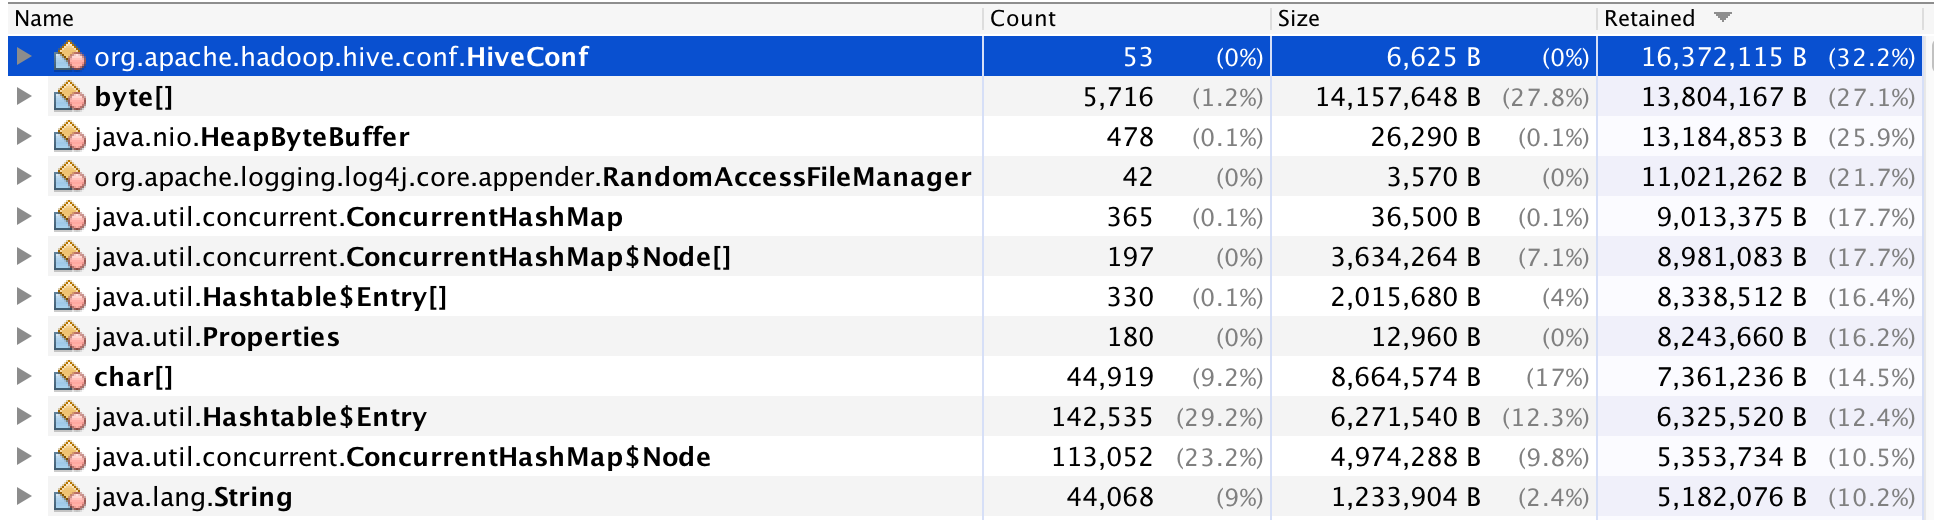
\includegraphics[width=150mm, keepaspectratio]{figures/hiveconf_memory.png}
	\centering
	\caption{Object with the most retained memory}
\end{figure}

For each session, an individual HiveConf object is created, which contains all the configuration properties of Hive. These configurations can easily contain thousands of values so the big heap memory is not that surprising. The first thing I recognized during the analyzis of the heap dump, is that each HiveConf object of a session use the same amount of memory. Thus, these objects cannot be that different from each other. If that is the case, why do we have a different one for every session?

The HiveConf class is a descendant of the \textit{Configuration.java} class, that is inherited from Hadoop. The biggest memory of each HiveConf a private Properties field. The Properties class is a type of HashMap that only contains String keys and values. Looking into the Properties fields of each HiveConf confirmed my assumption: they have exactly the same values apart from a few properties.

This inspired me to look more into the details. How these configuration objects are used? When we start Hive, Hadoop configuration properties are applied, and we read Hive's configuration file (hive-site.xml) and overlay those properties. After this, for each session we create a new HiveConf instance with copying the existing "base". This way sessions can add their own unique Properties to their configuration object. 

It is important to notice that we rarely touch the "base" configurations. Usually the sessions add some Properties to it and the base configuration remains untouched. To get rid of the memory overhead, a possible solution would be to use the same Properties object for each HiveConf if the values in them are the same.

\section{HIVE-20760: Reducing memory overhead due to multiple HiveConfs}
I already saw a somewhat similar problem, when looking into the partition memory issues. PartitionDesc used exactly the same Properties object, and the solution for that was introducing CopyOnFirstWriteProperties class \cite{hive-partitions}. 

It is a special subclass of Properties, designed to save memory when lots of identical Properties are created. The class uses interning to solve the problem: it has an interned Properties field which points to the same object for all instances that has identical contents. If any mutating method (\eg setProperties, put, clear) is called on the object, the content is copied to "this" instance, and we no longer use the interned object. 

As a first idea, I thought that using this class would help. However, HiveConfs are used differently from PartitionDesc, and this solution was desinged for that. We often call mutating methods on the Properties field of HiveConf. Each session is able to add additional values to its configuration. Thus, other solution is needed to save memory in this scenario, since using CopyOnFirstWriteProperties immediately throws away the interned Properties if we add a new property to it.

\subsection{Introducing HiveConfProperties class}
My idea was to intern only the "base" Properties. When we create a HiveConf from an already existing one using its "copy constuctor", instead of creating a built in \textit{java.util.Properties} we will use a subclass of Properties. I named this class HiveConfProperties. 

I designed HiveConfProperties to save memory caused by the many nearly individual HiveConfs. Right after we create a HiveConfProperties instance, from an already existing Properties, we can intern that. For interning, I used \textit{com.google.common.collect.Interner}. 

\subsubsection{How interning works} 
 When we have an object that we want to intern, we search for it in the "object pool" to see if there is already an object equal to the corresponding one. If we find one, we will use that in the future. If there is no object equal to the actual one then we put the object into the pool and then use it. Fortunately, there is already an existing implementation of this interning method in the Google Guava core java library.
 
 \subsubsection{How HiveConfProperties works}
 I divided the Properties object into two parts: an interned part, which contains the base Properties, and since we descend from \textit{the java.util.Properties}, we can use the "this" object to store properties as well.
 
 \begin{figure}[H]
 	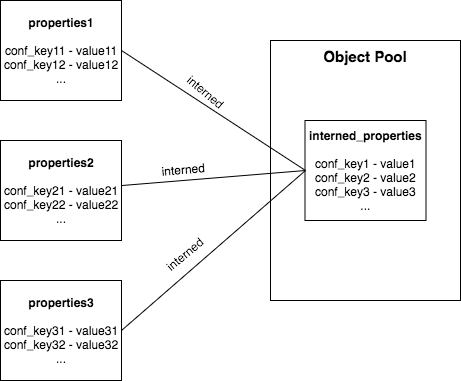
\includegraphics[width=100mm,keepaspectratio]{figures/hiveconf_solution.png}
 	\centering
 	\caption{How HiveConfProperties works}
 \end{figure}

\begin{lstlisting}
private Properties interned;

private Properties removed;
private int duplicatedPropertiesCount;

private static Interner<Properties> interner = Interners.newWeakInterner();

public HiveConfProperties(Properties p) {
	if(p != null) {
		interned = interner.intern(p);
	}
	removed =  new Properties();
	duplicatedPropertiesCount=0;
}
\end{lstlisting}

The code above is responsible for creating a HiveConfProperties instance. It stores the interned (base) Properties in a private field. Right after we want to construct an instance, we intern the given Properties object. The process that \textit{interner.intern(...)} does is explained above. A null check is also a must when we create a new HiveConfProperties, since calling the constructor with null parameter is possible in the code. I found this possibility when I submitted the patch to Apache Hive Jira and "PreCommit" tests failed during the Jenkins build. The \textit{removed} and the \textit{duplicatedPropertiesCount} field is needed for the interning to work as expected. 

If someone calls \textit{HiveConf.unset} funciton, \textit{Properties.remove} (this case \textit{HiveConfProperties.remove} will be called. If the property we want to remove is contained by the interned Properties object, we cannot remove it directly, because other HiveConfProperties may use it. To solve this issue, I introduced the \textit{removed} Properties field to store those values that should no longer be available. So if we want to get the value of a key, we first check if the key is in the \textit{removed} Properties: if the answer is yes, we will consider this property unavailable.

Duplications can occur in my solution: if someone would like to set a property, that is already in the \textit{interned} field, we cannot override it there, so we should add it in the non-interned Properties to return the correct value. However, this way we will have two properties with the same content. Calculating the size of the HashMap will be inaccurate. For solving this issue, I created a counter field called \textit{duplicatedPropertiesCount} to store the number of the duplicates. Knowing this value will allow us to provide an accurate size. 

Since HiveConfProperties is a subclass of \textit{java.util.Properties} and because of it subclass of \textit{java.util.HashTable}, I provided implementation of its methods.  \textit{hadoop.conf.Configuration} (base class of HiveConf) and \textit{HiveConf} only uses a subset of these functions, so I decided to implement only those, that can be invoked. For the other methods I will throw a \textit{NotImplementedException}. 

\subsection{Overriden functions of Properties}
\subsubsection{getProperty}
\begin{lstlisting}
@Override
public String getProperty(String key) {
	String property = super.getProperty(key);
	if (property == null) {
		if(interned != null && !removed.containsKey(key)) {
			property = interned.getProperty(key);
		}
	}
	return property;
}
\end{lstlisting}

If non-interned (super) contains the key, return that value. If not, we need to check if it is not in the \textit{removed} Properties (still valid). If the value is valid, return it from the base (interned). \textit{getProperty(String key, String defaultValue)} and \textit{get} method from HashTable works the same way. 
\subsubsection{setProperty}
\begin{lstlisting}
@Override
public synchronized Object setProperty(String key, String value) {
	if(interned != null && interned.containsKey(key) && !super.containsKey(key)) {
		String internedValue = interned.getProperty(key);
		if(internedValue.equals(value)) {
			return internedValue;
		}
		duplicatedPropertiesCount++;
	}
	//If removed contains this key, and we want to set it, it is no longer "removed"
	if(removed.containsKey(key)) {
		removed.remove(key);
	}
	return super.setProperty(key, value);
}
\end{lstlisting}

If interned already contains the property to be set, we need to set it in the non-interned Properties. However, this way we will have duplicates, since both Properties instance will contain the same value. Thus, to be able to give a correct size when needed, we need to count these duplicates. If we are setting a value, that had been removed previously, we need to "revalidate" the property. If the value is not changed, we should not set it in the non-interned Properties to avoid unnecessary duplicates. 

\subsubsection{mergeProperties helper function}
To override functions such as \textit{stringPropertyNames} or \textit{keySet} \etc I introduced a helper function. Since for these methods, we need values of the properties from both (non-interned and interned) objects, the helper method will merge the two parts into one Properties. This way we can just delegate the call to the merge Properties object. In the \textit{mergeProperties} I simply iterated through both parts and collected each HashTable entry (if not removed) and returned a new Properties instance. 

Overriding for example the keySet function will look like this:
\begin{lstlisting}
@Override
public Set<Object> keySet() {
	return mergeProperties().keySet();
}
\end{lstlisting}

We can do the same for all the functions where merging is needed: \textit{keys, entrySet, stringPropertyNames, toString \etc}

\subsubsection{size}
\begin{lstlisting}
@Override
public synchronized int size() {
	if(interned != null) {
		return super.size() + interned.size() - duplicatedPropertiesCount - removed.size();
	}
	return super.size();
}
\end{lstlisting}
The size of HiveConfProperties is the size of interned + size of non-interned - \textit{duplicatedPropertiesCount}. We have to subtract the \textit{duplicatedPropertiesCount}, because duplicates can happen.Also we have to subtract the size of the removed Properties, since those had been removed.

\subsubsection{containsKey, containsValue}
\begin{lstlisting}
@Override
public synchronized boolean containsKey(Object key) {
	if(interned != null) {
		return !removed.containsKey(key) && (super.containsKey(key) || interned.containsKey(key));
	}
	return super.containsKey(key);
}
\end{lstlisting}
A key or value is contained by a HiveConfProperties instance, if its removed field does not contain it and the interned or non-interned does.

\subsubsection{remove}
\begin{lstlisting}
@Override
public synchronized Object remove(Object key) {
	if(interned != null) {
		if (interned.containsKey(key)) {	
			String v = interned.getProperty((String) key);
			removed.setProperty((String) key, v);
			return v;
		}
	}
	return super.remove(key);
}
\end{lstlisting}
We cannot remove the property from the interned Properties (other HiveConfs may use it). We store the value in the \textit{removed} Properties field and in the future the properties stored there will not be valid. If we would like to remove a value from the non-interned field, we can simply do that, since it will not affect any other HiveConfProperties instance.

\subsubsection{equals}
Maybe the most complicated method is the \textit{equals} inherited from the HashTable class. Deciding whether an object is equal to another or not should be fast. Merging the two parts can be slow if equals is used widely. Thus, I followed the way that HashTable's equals method works. It is possible to call equals on a HiveConfProperties object but giving a simple \textit{java.util.Properties}. The equals method should also work correctly in this scenario. I will not include the code for \textit{equals} method, because it is to big, and nothing complicated is done there, but the code can be found in the Jira for the issue \cite{hive-conf}.

If other Properties object is a HiveConfProperties, with the help of \textit{instanceof} keyword we can decide whether the other Properties is a HiveConfProperties or not. If the answer is positive, we need to check its interned Properties object as well. As a first step we check their sizes. If they are not equal, we can return false immediately. If sizes are equal, first we will iterate through the non-interned Properties in the "this" object. For each HashTable entries we will check two things: if value is null in the entry, "other" HiveConfProperties should not contain the key, otherwise the two object cannot be the same, so we can return false. If value for the entry is not null, value from "this" should be equal to value from the other object. 

If all entries from the non-interned Properties are contained by the other Properties object. We still need to check the same for this.interned Properties. The code will be the same expect, we will iterate through the entries of the interned Properties. 

The code is simpler if the other object is not a HiveConfProperties. We do not need the check two parts. We can just iterate through the entries of the "other" Properties and do the same checks as mentioned before.

\subsection{Applying the solution in HiveConf}
HiveConf is a descendant of Configuration class, which comes from the Hadoop Common library. The properties field that is causing the memory overhead is also in the base class and its visibility is private. We have two options to resolve this:
\begin{enumerate}
	\item Change the visibility of properties field to protected, so in HiveConf we can change the type of the field to HiveConfProperties simply
	\item Continue to use private visibility, and change the type of the field in HiveConf using reflection.
\end{enumerate}

Changing the visibility in Hadoop may not be the ideal design choice, since Hive should depend on Hadoop and not the other way around. I decided to change the type using reflection in Hive side. 

\begin{lstlisting}
try {
	Field propertiesField = FieldUtils.getDeclaredField(HiveConf.class.getSuperclass(), "properties", true);
	if(!(propertiesField.get(other) instanceof HiveConfProperties)) {
		HiveConfProperties properties = new HiveConfProperties((Properties) propertiesField.get(this));
		FieldUtils.writeField(this, "properties", properties, true);
	}
}  catch (IllegalAccessException e) {
	e.printStackTrace();
}
\end{lstlisting}

I used \textit{FieldUtils} class from \textit{commons-lang} library to access the properties field in the superclass and change reapply the Properties object wrapped in a HiveConfProperties.

HiveConf has an additional Properties object called \textit{origProp}. The values contained by the \textit{origProp} objects for different HiveConfs are also very similar, so interning those as well would also remove some memory overhead. 

\subsection{Memory win by the change}
\begin{figure}[H]
	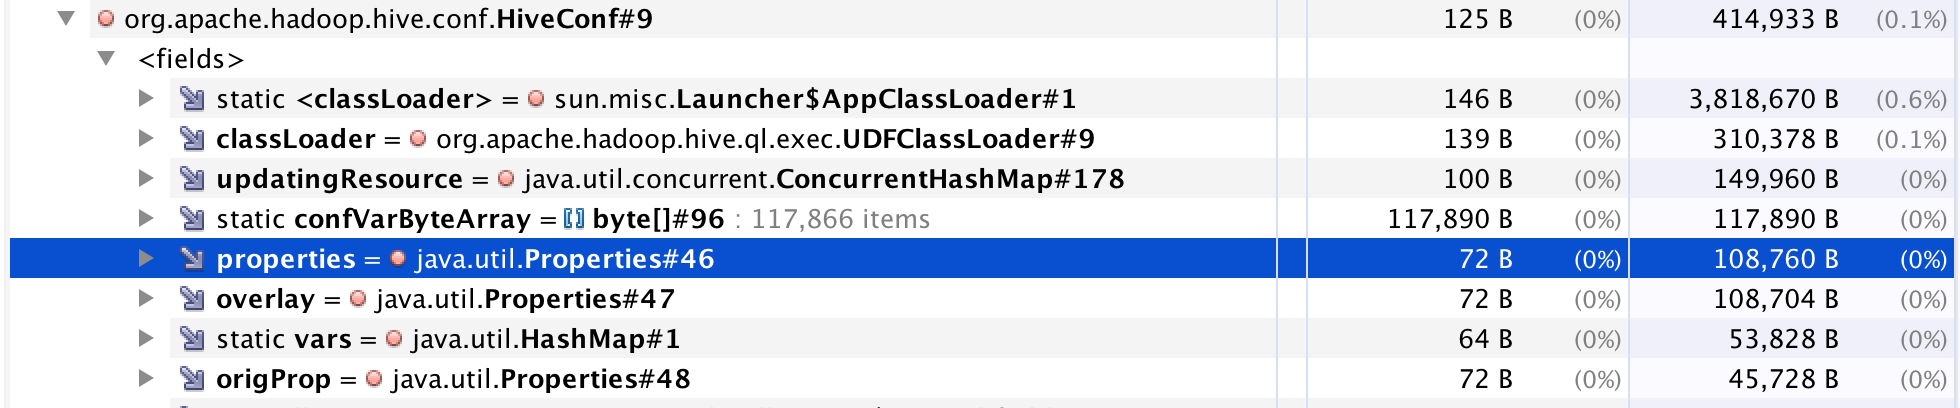
\includegraphics[width=150mm, keepaspectratio]{figures/hiveconf_orig.png}
	\centering
	\caption{Before using HiveConfProperties}
\end{figure}

\subsection{Memory win by the change}
\begin{figure}[H]
	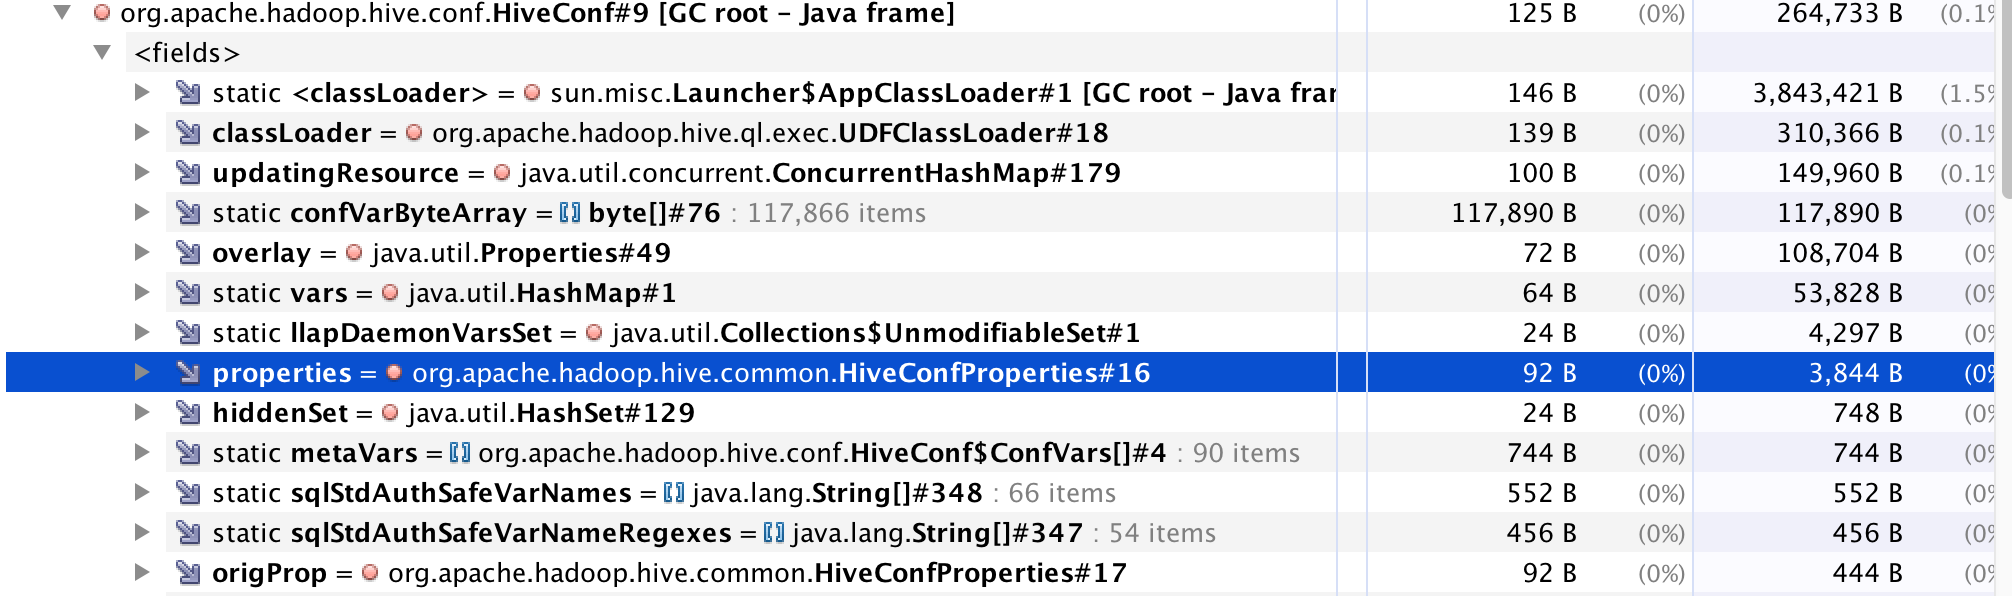
\includegraphics[width=150mm, keepaspectratio]{figures/hiveconf_interned.png}
	\centering
	\caption{After using HiveConfProperties}
\end{figure}

Comparing the heap dumps shows the benefits of interning the Properties in HiveConf. Without the use of HiveConfProperties one configuration object conaining 1910 properties used around 415 Kilobytes. With the use of HiveConfProperties it was reduced to 265 Kilobytes.It is nearly 40\% memory saved for each HiveConf. 

When we use Hive on Spark running with a large number of cores per executor, we have about 10\% of memory overhead due to multiple HiveConfs . This can be reduced significantly using my solution. 

\section{Future work around configuration objects}
The issue I reported is  still ongoing, since tests are needed to see if my patch works correctly in every scenario. I also provided a test class, which needs to be expanded, to cover all the scenarios a Properties object can be used by HiveConf. 

Hadoop also has an implementation of the Configuration class, called JobConf. These objects are also present in HS2 and causes memory overhead the same way as HiveConf does. There is an open source Jira that was intended to solve the duplication without getting \textit{ConcurrentModificationException}, but the memory problem was not resolved just prevented throwing the exception \cite{hive-jobconf}. The solution I provide for HiveConf could also be used for getting rid of the duplication in JobConf.